%% LyX 2.3.7 created this file.  For more info, see http://www.lyx.org/.
%% Do not edit unless you really know what you are doing.
\documentclass[journal,article,submit,pdftex,moreauthors]{Definitions/mdpi}
\usepackage[utf8]{inputenc}
\usepackage{array}
\usepackage{float}
\usepackage{booktabs}
\usepackage{url}
\usepackage{amsmath}
\usepackage{graphicx}

\makeatletter

%%%%%%%%%%%%%%%%%%%%%%%%%%%%%% LyX specific LaTeX commands.

\Title{Refining the Eel and Grouper Optimizer with Intelligent Modifications
for Global Optimization}

\TitleCitation{Refining the Eel and Grouper Optimizer with Intelligent Modifications
for Global Optimization}

\Author{Glykeria Kyrou$^{1}$, Vasileios Charilogis$^{2}$ and Ioannis G.
Tsoulos$^{3,*}$}

\AuthorNames{Glykeria Kyrou, Vasileios Charilogis and Ioannis G. Tsoulos }

\AuthorCitation{Kyrou, G.; Charilogis, V.; Tsoulos, I.G. }


\address{$^{1}$\quad{}Department of Informatics and Telecommunications,
University of Ioannina, 47150 Kostaki Artas, Greece; g.kyrou@uoi.gr\\
$^{2}$\quad{}Department of Informatics and Telecommunications, University
of Ioannina, 47150 Kostaki Artas, Greece; v.charilog@uoi.gr\\
$^{3}\quad$Department of Informatics and Telecommunications, University
of Ioannina, 47150 Kostaki Artas, Greece;itsoulos@uoi.gr}


\corres{Correspondence: itsoulos@uoi.gr}


\abstract{Global optimization is used in many practical and scientific problems.
For this reason, various computational techniques have been developed.
Particularly important are the evolutionary techniques, which simulate
natural phenomena with the aim of detecting the global minimum in
complex problems. A new evolutionary method is the Eel and Grouper
Optimization (EGO) algorithm, inspired by the symbiotic relationship
and foraging strategy of eels and groupers in marine ecosystems. In
the present work, a series of improvements are proposed that aim both
at the efficiency of the algorithm to discover the total minimum of
multidimensional functions and at the reduction of the required execution
time through the effective reduction of the number of functional evaluations.
These modifications include the incorporation of a stochastic termination
technique as well as an improvement sampling technique.\textbf{ }The
proposed modifications have been tested on multidimensional functions
available from the relevant literature and compared with other evolutionary
methods.}


\keyword{Global optimization; Metaheuristic algorithms; Stochastic methods;
Evolutionary algorithms; Swarm algorithms; Termination strategies;
Sampling techniques.}

\newcommand*\LyXZeroWidthSpace{\hspace{0pt}}
\DeclareTextSymbolDefault{\textquotedbl}{T1}
%% Because html converters don't know tabularnewline
\providecommand{\tabularnewline}{\\}
\floatstyle{ruled}
\newfloat{algorithm}{tbp}{loa}
\providecommand{\algorithmname}{Algorithm}
\floatname{algorithm}{\protect\algorithmname}

%%%%%%%%%%%%%%%%%%%%%%%%%%%%%% User specified LaTeX commands.
%  LaTeX support: latex@mdpi.com 
%  For support, please attach all files needed for compiling as well as the log file, and specify your operating system, LaTeX version, and LaTeX editor.

%=================================================================


% For posting an early version of this manuscript as a preprint, you may use "preprints" as the journal and change "submit" to "accept". The document class line would be, e.g., \documentclass[preprints,article,accept,moreauthors,pdftex]{mdpi}. This is especially recommended for submission to arXiv, where line numbers should be removed before posting. For preprints.org, the editorial staff will make this change immediately prior to posting.

%--------------------
% Class Options:
%--------------------
%----------
% journal
%----------
% Choose between the following MDPI journals:
% acoustics, actuators, addictions, admsci, adolescents, aerospace, agriculture, agriengineering, agronomy, ai, algorithms, allergies, alloys, analytica, animals, antibiotics, antibodies, antioxidants, applbiosci, appliedchem, appliedmath, applmech, applmicrobiol, applnano, applsci, aquacj, architecture, arts, asc, asi, astronomy, atmosphere, atoms, audiolres, automation, axioms, bacteria, batteries, bdcc, behavsci, beverages, biochem, bioengineering, biologics, biology, biomass, biomechanics, biomed, biomedicines, biomedinformatics, biomimetics, biomolecules, biophysica, biosensors, biotech, birds, bloods, blsf, brainsci, breath, buildings, businesses, cancers, carbon, cardiogenetics, catalysts, cells, ceramics, challenges, chemengineering, chemistry, chemosensors, chemproc, children, chips, cimb, civileng, cleantechnol, climate, clinpract, clockssleep, cmd, coasts, coatings, colloids, colorants, commodities, compounds, computation, computers, condensedmatter, conservation, constrmater, cosmetics, covid, crops, cryptography, crystals, csmf, ctn, curroncol, currophthalmol, cyber, dairy, data, dentistry, dermato, dermatopathology, designs, diabetology, diagnostics, dietetics, digital, disabilities, diseases, diversity, dna, drones, dynamics, earth, ebj, ecologies, econometrics, economies, education, ejihpe, electricity, electrochem, electronicmat, electronics, encyclopedia, endocrines, energies, eng, engproc, ent, entomology, entropy, environments, environsciproc, epidemiologia, epigenomes, est, fermentation, fibers, fintech, fire, fishes, fluids, foods, forecasting, forensicsci, forests, foundations, fractalfract, fuels, futureinternet, futureparasites, futurepharmacol, futurephys, futuretransp, galaxies, games, gases, gastroent, gastrointestdisord, gels, genealogy, genes, geographies, geohazards, geomatics, geosciences, geotechnics, geriatrics, hazardousmatters, healthcare, hearts, hemato, heritage, highthroughput, histories, horticulturae, humanities, humans, hydrobiology, hydrogen, hydrology, hygiene, idr, ijerph, ijfs, ijgi, ijms, ijns, ijtm, ijtpp, immuno, informatics, information, infrastructures, inorganics, insects, instruments, inventions, iot, j, jal, jcdd, jcm, jcp, jcs, jdb, jeta, jfb, jfmk, jimaging, jintelligence, jlpea, jmmp, jmp, jmse, jne, jnt, jof, joitmc, jor, journalmedia, jox, jpm, jrfm, jsan, jtaer, jzbg, kidney, kidneydial, knowledge, land, languages, laws, life, liquids, literature, livers, logics, logistics, lubricants, lymphatics, machines, macromol, magnetism, magnetochemistry, make, marinedrugs, materials, materproc, mathematics, mca, measurements, medicina, medicines, medsci, membranes, merits, metabolites, metals, meteorology, methane, metrology, micro, microarrays, microbiolres, micromachines, microorganisms, microplastics, minerals, mining, modelling, molbank, molecules, mps, msf, mti, muscles, nanoenergyadv, nanomanufacturing, nanomaterials, ncrna, network, neuroglia, neurolint, neurosci, nitrogen, notspecified, nri, nursrep, nutraceuticals, nutrients, obesities, oceans, ohbm, onco, oncopathology, optics, oral, organics, organoids, osteology, oxygen, parasites, parasitologia, particles, pathogens, pathophysiology, pediatrrep, pharmaceuticals, pharmaceutics, pharmacoepidemiology, pharmacy, philosophies, photochem, photonics, phycology, physchem, physics, physiologia, plants, plasma, pollutants, polymers, polysaccharides, poultry, powders, preprints, proceedings, processes, prosthesis, proteomes, psf, psych, psychiatryint, psychoactives, publications, quantumrep, quaternary, qubs, radiation, reactions, recycling, regeneration, religions, remotesensing, reports, reprodmed, resources, rheumato, risks, robotics, ruminants, safety, sci, scipharm, seeds, sensors, separations, sexes, signals, sinusitis, skins, smartcities, sna, societies, socsci, software, soilsystems, solar, solids, sports, standards, stats, stresses, surfaces, surgeries, suschem, sustainability, symmetry, synbio, systems, taxonomy, technologies, telecom, test, textiles, thalassrep, thermo, tomography, tourismhosp, toxics, toxins, transplantology, transportation, traumacare, traumas, tropicalmed, universe, urbansci, uro, vaccines, vehicles, venereology, vetsci, vibration, viruses, vision, waste, water, wem, wevj, wind, women, world, youth, zoonoticdis 

%---------
% article
%---------
% The default type of manuscript is "article", but can be replaced by: 
% abstract, addendum, article, book, bookreview, briefreport, casereport, comment, commentary, communication, conferenceproceedings, correction, conferencereport, entry, expressionofconcern, extendedabstract, datadescriptor, editorial, essay, erratum, hypothesis, interestingimage, obituary, opinion, projectreport, reply, retraction, review, perspective, protocol, shortnote, studyprotocol, systematicreview, supfile, technicalnote, viewpoint, guidelines, registeredreport, tutorial
% supfile = supplementary materials

%----------
% submit
%----------
% The class option "submit" will be changed to "accept" by the Editorial Office when the paper is accepted. This will only make changes to the frontpage (e.g., the logo of the journal will get visible), the headings, and the copyright information. Also, line numbering will be removed. Journal info and pagination for accepted papers will also be assigned by the Editorial Office.

%------------------
% moreauthors
%------------------
% If there is only one author the class option oneauthor should be used. Otherwise use the class option moreauthors.

%---------
% pdftex
%---------
% The option pdftex is for use with pdfLaTeX. If eps figures are used, remove the option pdftex and use LaTeX and dvi2pdf.

%=================================================================
% MDPI internal commands - do not modify
\firstpage{1} 
 
\setcounter{page}{\@firstpage} 

\pubvolume{1}
\issuenum{1}
\articlenumber{0}
\pubyear{2024}
\copyrightyear{2024}
%\externaleditor{Academic Editor: Firstname Lastname} % For journal Automation, please change Academic Editor to "Communicated by"
\datereceived{}
\daterevised{ } % Comment out if no revised date
\dateaccepted{}
\datepublished{}
%\datecorrected{} % Corrected papers include a "Corrected: XXX" date in the original paper.
%\dateretracted{} % Corrected papers include a "Retracted: XXX" date in the original paper.
\hreflink{https://doi.org/} % If needed use \linebreak
%\doinum{}
%------------------------------------------------------------------
% The following line should be uncommented if the LaTeX file is uploaded to arXiv.org
%\pdfoutput=1

%=================================================================
% Add packages and commands here. The following packages are loaded in our class file: fontenc, inputenc, calc, indentfirst, fancyhdr, graphicx, epstopdf, lastpage, ifthen, lineno, float, amsmath, setspace, enumitem, mathpazo, booktabs, titlesec, etoolbox, tabto, xcolor, soul, multirow, microtype, tikz, totcount, changepage, attrib, upgreek, cleveref, amsthm, hyphenat, natbib, hyperref, footmisc, url, geometry, newfloat, caption

%=================================================================
%% Please use the following mathematics environments: Theorem, Lemma, Corollary, Proposition, Characterization, Property, Problem, Example, ExamplesandDefinitions, Hypothesis, Remark, Definition, Notation, Assumption
%% For proofs, please use the proof environment (the amsthm package is loaded by the MDPI class).

%=================================================================
% The fields PACS, MSC, and JEL may be left empty or commented out if not applicable
%\PACS{J0101}
%\MSC{}
%\JEL{}

%%%%%%%%%%%%%%%%%%%%%%%%%%%%%%%%%%%%%%%%%%
% Only for the journal Diversity
%\LSID{\url{http://}}

%%%%%%%%%%%%%%%%%%%%%%%%%%%%%%%%%%%%%%%%%%
% Only for the journal Applied Sciences:
%\featuredapplication{Authors are encouraged to provide a concise description of the specific application or a potential application of the work. This section is not mandatory.}
%%%%%%%%%%%%%%%%%%%%%%%%%%%%%%%%%%%%%%%%%%

%%%%%%%%%%%%%%%%%%%%%%%%%%%%%%%%%%%%%%%%%%
% Only for the journal Data:
%\dataset{DOI number or link to the deposited data set in cases where the data set is published or set to be published separately. If the data set is submitted and will be published as a supplement to this paper in the journal Data, this field will be filled by the editors of the journal. In this case, please make sure to submit the data set as a supplement when entering your manuscript into our manuscript editorial system.}

%\datasetlicense{license under which the data set is made available (CC0, CC-BY, CC-BY-SA, CC-BY-NC, etc.)}

%%%%%%%%%%%%%%%%%%%%%%%%%%%%%%%%%%%%%%%%%%
% Only for the journal Toxins
%\keycontribution{The breakthroughs or highlights of the manuscript. Authors can write one or two sentences to describe the most important part of the paper.}

%%%%%%%%%%%%%%%%%%%%%%%%%%%%%%%%%%%%%%%%%%
% Only for the journal Encyclopedia
%\encyclopediadef{Instead of the abstract}
%\entrylink{The Link to this entry published on the encyclopedia platform.}
%%%%%%%%%%%%%%%%%%%%%%%%%%%%%%%%%%%%%%%%%%

%%%%%%%%%%%%%%%%%%%%%%%%%%%%%%%%%%%%%%%%%%
% Only for the journal Advances in Respiratory Medicine
%\addhighlights{yes}
%\renewcommand{\addhighlights}{%

%\noindent This is an obligatory section in “Advances in Respiratory Medicine”, whose goal is to increase the discoverability and readability of the article via search engines and other scholars. Highlights should not be a copy of the abstract, but a simple text allowing the reader to quickly and simplified find out what the article is about and what can be cited from it. Each of these parts should be devoted up to 2~bullet points.\vspace{3pt}\\
%\textbf{What are the main findings?}
% \begin{itemize}[labelsep=2.5mm,topsep=-3pt]
% \item First bullet.
% \item Second bullet.
% \end{itemize}\vspace{3pt}
%\textbf{What is the implication of the main finding?}
% \begin{itemize}[labelsep=2.5mm,topsep=-3pt]
% \item First bullet.
% \item Second bullet.
% \end{itemize}
%}
%%%%%%%%%%%%%%%%%%%%%%%%%%%%%%%%%%%%%%%%%%

\makeatother

\begin{document}
\maketitle

\section{Introduction}

The goal of global optimization method aims to discover the global
minimum of a continuous multidimensional function, and it is defined
as
\begin{equation}
x^{*}=\mbox{arg}\min_{x\in S}f(x)\label{eq:eq1}
\end{equation}
with $S$: 
\[
S=\left[a_{1},b_{1}\right]\times\left[a_{2},b_{2}\right]\times\ldots\left[a_{n},b_{n}\right]
\]
The function $f(x)$ is defined as $f:S\rightarrow R,S\subset R^{n}$
and the set $S$ denotes the bounds of $x$. of In recent years many
researchers have published important reviews on global optimization
\citep{plhroforikh,computer,computer1}. Global optimization is a
technique of vital importance in many fields of science and applications,
as it allows finding the optimal solution to problems with multiple
local solutions. In mathematics \citep{maths,maths-1,maths2,key-maths3},
it is used to solve complex mathematical problems, in physics \citep{fusikh,fusikh1,fysikhh},
it is used to analyze and improve models that describe natural phenomena,
in chemistry \citep{xhmeia,xhmeia1,xhmeia2}, it analyzes and designs
molecules and chemical diagnostic tools, and in medicine\citep{medicine}
it analyzes and designs therapeutic strategies and diagnostic tools
.

The methods that aim to discover the global minimum has two main categories,
deterministic \citep{determistic,determistic1,determistic2} and stochastic
\citep{stohastic,stohastic1,stohastic2}.\textbf{ }In the first category,
there are techniques aimed at identifying the total minimum with some
certainty, such as interval methods \citep{key-1,interval2} and are
usually distinguished by their complex implementation. The vast majority
of global optimization algorithms belong to \LyXZeroWidthSpace\LyXZeroWidthSpace stochastic
methods that have simpler implementation and can also be applied to
large - scale problems. Recently, Sergeyev et al \citep{Sergeyev}
published a systematic comparison between deterministic and stochastic
methods for global optimization problems.

An important branch of the stochastic methods are the evolutionary
methods, that attempt to mimic a series of natural processes. Among
these methods one can find the Differential Evolution method \citep{diffe1,diffe2},
Particle Swarm Optimization (PSO) methods \citep{pso_major,pso1,pso2},
Ant Colony optimization methods \citep{aco1,aco2}, Genetic algorithms
\citep{genetic1,genetic2}, the Exponential Distribution Optimizer
\citep{edo}, the Brain Storm Optimization method \citep{bdo} etc.
Additionally, since in recent years there has been an extremely wide
spread of parallel computing units, many researches have proposed
evolutionary methods that exploit modern parallel processing units
\citep{gpu1,gpu2,gpu3}. 

Among the evolutionary techniques one finds a large group of methods
that have been explored intensively in recent years, the so - called
Swarm Intelligence algorithms. These methods \citep{swarm1,swarm2,swarm}
are inspired by the collective behavior of swarm. These algorithms
mimic systems in which candidate solutions interact locally and cooperate
worldwide to discover the global minimum of any problem. These algorithms
are very important tools for dealing with complex optimization problems
in many applications \citep{APPS}. 

In addition to the previously mentioned Particle Swarm Optimization
and Ant Colony methods techniques that are also included in Swarm
intelligence algorithms, other methods that belong to this category
are, the Fast Bacterial Swarming Algorithm (FBSA) \citep{bacterial},
the Fish Swarm Algorithm \citep{fish}, the Dolphin Swarm Algorithm
\citep{dolphin}, the Whale Optimization Algorithm (WOA) algorithm
\citep{WOA,WOA1,WOA2,WOA3}, the Tunicate Swarm Algorithm \citep{tunicate},
the Salp Swarm algorithm (SSA) algorithm \citep{ssaa,SSA,SSA1,SSA2},
the Artificial Bee Colony algorithm \citep{abc} etc. These methods
simulate a series of complex interactions between biological species
\citep{search algorithm,several metaheuristic algorithms }, such
as:
\begin{enumerate}
\item Naturalism: Where two species can live without affecting each other. 
\item Predation, where one creature dies by feeding another. 
\item Parasitism: where one species can cause harm to another. 
\item In competitive mode, the same or different organizations compete for
resources. 
\item Mutualism \citep{mutualism-parasitism,mutualistic,Competition in mutualistic systems}:
when two organisms have a beneficial interaction. 
\end{enumerate}
Among swarm intelligence algorithms one can find the Eel and Grouper
(EGO) algorithm, which is inspired by the symbiotic interaction and
foraging strategy of eels and groupers in marine ecosystems.\textbf{
}Bshary et al. \citep{hunting between groupers and giant moray eels in the Red Sea}
consider that target ingestion, something observed in eels and groupers,
is a necessary condition for interspecific cooperative hunting to
occur. Intraspecific predation could increase the hunting efficiency
of predators by mammals. According to Ali Mohammadzadeh and Seyedali
Mirjalili the EGO optimization algorithm \citep{Eel and grouper optimizer}
generates a set of random answers, then stores the best answers found
so far, allocates them to the target point, and changes the answers
with them. As the number of iterations increases, the limits of the
sine function are changed to enhance the phase of finding the best
solution. This method stops the process when the iteration exceeds
the maximum number. Because the EGO optimization algorithm generates
and boosts a collection of random responses, it has the advantage
of increased local optimum discovery and avoidance compared to individual
methods. According to Ali Mohammadzadeh and Seyedali Mirjalili, the
algorithm’s capabilities extend to NP-hard problems in wireless sensor
networks\citep{key-28}, IoT\citep{key-29}, logistics\citep{key-30},
smart agriculture\citep{key-34}, bioinformatics\citep{key-35} and
machine learning\citep{key-36} in various fields such as programming,
image segmentation\citep{key-37}, electrical circuit design\citep{key-38},
feature selection and 3D path planning in robotics\citep{key-39}. 

This paper introduces some modifications to the EGO algorithm in order
to improve its efficiency. The proposed amendments are presented below:
\begin{itemize}
\item The addition of a sampling technique based on the K-means method \citep{kmeans2,kmeans-ereunhtikh-koinothta,MacQueen}.
The sampling points will facilitate finding the global minimum of
the function in the most efficient way. Additionally, by applying
this method, nearby points are discarded. Initialization of the population
of evolutionary techniques is a crucial factor which may accelarate
the\textbf{. }The initialization of populations in evolutionary techniques
can push these techniques to more efficiently locate the global minimum,
and in this direction a multitude of research works have been presented
in recent years, such as the work of Maaranen et al \citep{gainit1},
where they apply quasi-random sequences in the initial population
of a genetic algorithm. Likewise, Paul et al \citep{gainit2} suggested
a method for the initialization of the population of genetic algorithms
using a Vari-begin and Vari-diversity (VV) seeding method. Ali et
al. proposed a series of initialization methods for the Differential
Evolution method \citep{aliInit}. A novel method that initializes
the population of evolutionary algorithms using clustering and Cauchy
deviates is suggested in the work of Bajer et al \citep{bajerInit}.
A systematic review of initialization techniques for evolutionary
algorithms can be found in the work of Kazimipour et al \citep{KazimipourInit}.
\item Using a termination technique that is developed with random measurements.
Each time the algorithm is repeated, the minimum value is recorded.
When this remains constant for a pre - defined number of iterations,
the process is terminated. Therefore, the method will terminated without
wasting execution time in iterations, avoiding unnecessary consumption
of computing resources. There are several methods found in the recent
bibliography to terminate optimization methods. An overview of methods
used to terminate evolutionary algorithms can be found in the work
of Jain et al \citep{jainTermination}. Also, Zielinski et al outlined
some stopping rules used particularly in the Differential Evolution
method \citep{zilTermination}. Recently, Ghoreishi et al. published
a literature study concerning various termination criteria on evolutionary
algorithms \citep{ghoreishiTermination}. Moreover, Ravber et al.
performed an extended research on the impact of maximum number of
iterations to the effectiveness of evolutionary algorithms \citep{ravberTermination}.
\item Application of randomness in the definition of the range of the positions
of candidate solutions.
\end{itemize}
The rest of this paper is divided into the following sections: in
section \ref{sec:Materials-and-Methods}, the proposed method is fully
described, in section \ref{sec:Results} the experimental results
and statistical comparisons are outlined and finally in section \ref{sec:Conclusions}
some conclusions and guidelines for future improvements are discussed.

\section{The proposed method\label{sec:Materials-and-Methods}}

The main steps of the proposed algorithm are discussed in this section.
Also, the mentioned modifications are fully described.

\subsection{The main steps of the algorithm\label{subsec:The-main-steps}}

EGO optimization algorithm starts by initializing a population consisting
of \textquotedbl search agents\textquotedbl{} that search to find
the optimal solution. At each iteration, the position of the \textquotedbl prey\textquotedbl{}
(optimal solution) is calculated. Agent positions are adjusted based
on random variables and their distance based on the optimal position.At
the end of each iteration, the current solutions are compared and
it is decided whether the algorithm should continue or terminate.
The steps of the proposed method are provided in Algorithm \ref{alg:EGO-Algorithm}.
Also, the algorithm is presented as a series of steps in the flowchart
of Figure \ref{fig:flowEgo}. Using flowchart and algorithm simultaneously
enhances visual perception and detailed analysis of logic and processes.

\textbf{}
\begin{algorithm}[H]
\textbf{Initialization step.}
\begin{enumerate}
\item \textbf{Define} as $N_{c}$ the number of elements in the search Agents
\item \textbf{Define} as $N_{g}$, the maximum number of allowed iterations.
\item \textbf{Initialize} randomly the search agents $x_{i},\ i=1,\ldots,N_{c}$
in set $S$. 
\item \textbf{Set} $t=0$, the iteration counter.
\item \textbf{Set} $s_{r}=0$, the starvation rate of the algorithm. 
\item \textbf{Set} $m=1$, this parameter influences how the variables $f_{1},f_{2}$
are defined, which in turn affects the calculation of new positions.
When $m=2$, it introduces randomness to the range of positions before
the update, while in the inactive state, the range remains fixed.
\end{enumerate}
\textbf{Calculation step.}
\begin{enumerate}
\item \textbf{While} termination criteria are not hold \textbf{do}
\begin{enumerate}
\item Update variables $a$ and $s_{r}$:
\begin{itemize}
\item \textbf{$a=2-2\frac{t}{N_{g}}$ }
\item \textbf{$s_{r}=100\frac{t}{N_{g}}$}
\end{itemize}
\item Compute the fitness of each search agents.
\item Sort all solutions according to their fitness values.
\item Set $\mbox{XP}$ the estimated position of the prey.
\item \textbf{For} $i=1,\ldots,N_{c}$ \textbf{do}
\begin{enumerate}
\item \textbf{Update }random variables\textbf{ $r_{1},r_{2},r_{3},r_{4},C_{1},C_{2},b\:$
:}
\begin{itemize}
\item \textbf{$r_{1}$}and $r_{2}$ are random numbers in $[0,1]$
\item \textbf{$r_{3}=(a-2)r_{1}+2$}
\item \textbf{$r_{4}=100r_{2}$ }
\item \textbf{$C_{1}=2*a*r_{1}-a$}
\item \textbf{$C_{2}=2*r_{1}$}
\item \textbf{$b=a*r_{2}$}
\item \textbf{Select} a random position $v\in\left\{ 1,\ldots,N_{c}\right\} $
\item \textbf{if $\left(r4\le s_{r}\right)$ then set $XE=C_{2}XP$ else
$XE=position[random\:index\:v]$ }
\end{itemize}
\item \textbf{Create} the vector $y=\left[y_{1,}y_{2},\ldots,y_{n}\right]$
with the following procedure
\item \textbf{For} $j=1,\ldots,n$ \textbf{do}
\begin{enumerate}
\item \textbf{Set$X_{1}=e^{br_{3}}\sin\left(2\pi r_{3}\right)C_{1}\left|\mbox{XE}-\mbox{XP}\right|+\mbox{XE},$
where $\mbox{XE}=C_{2}x_{i,j}$}
\item \textbf{Set $X_{2}=x_{i,j}+C_{1}\left|x_{i,j}-\mbox{XP}\right|$}
\item \textbf{if $m=1$ then set $f_{1}=0.8,f_{2}=0.2$ else set $f_{1}$
}to a random number in $[0,2]$ and $f_{2}$ to a random number in
$[-2,2]$
\item \textbf{Set} $p\in[0,1]$ a random number.
\item \textbf{if $\left(p\le0.5\right)$ then set $x_{i,j}=\frac{f_{1}X_{1}+f_{2}X_{2}}{2}$
else set $x_{i,j}=\frac{f_{2}X_{1}+f_{1}X_{2}}{2}$}
\end{enumerate}
\item \textbf{EndFor}
\end{enumerate}
\item \textbf{End For}
\end{enumerate}
\textbf{Termination check step}
\begin{enumerate}
\item \textbf{Set $t=t+1$}
\item \textbf{If $t\ge N_{g}$ terminate.}
\item \textbf{Else}
\item Calculate the stopping that proposed in the work of Charilogis \citep{charilogis}.
In the Similarity stopping rule, at every iteration t, the absolute
difference between the current located global minimum $f_{min}^{(t)}$
and the previous best value $f_{min}^{(t-1)}$ is calculated:
\end{enumerate}
\begin{centering}
\begin{equation}
\delta^{t}=\left|f_{\mbox{min}}^{(t)}-f_{\mbox{min}}^{(t-1)}\right|\label{eq:best}
\end{equation}
\par\end{centering}
The algorithm terminated when $\delta^{t}\le\epsilon$ for $N_{k}$
consecutive iterations, where $\epsilon$ is a small positive value.
\item \textbf{End While}
\item \textbf{\caption{EGO Algorithm\label{alg:EGO-Algorithm}}
}
\end{enumerate}
\end{algorithm}

\begin{figure}[H]
\begin{centering}
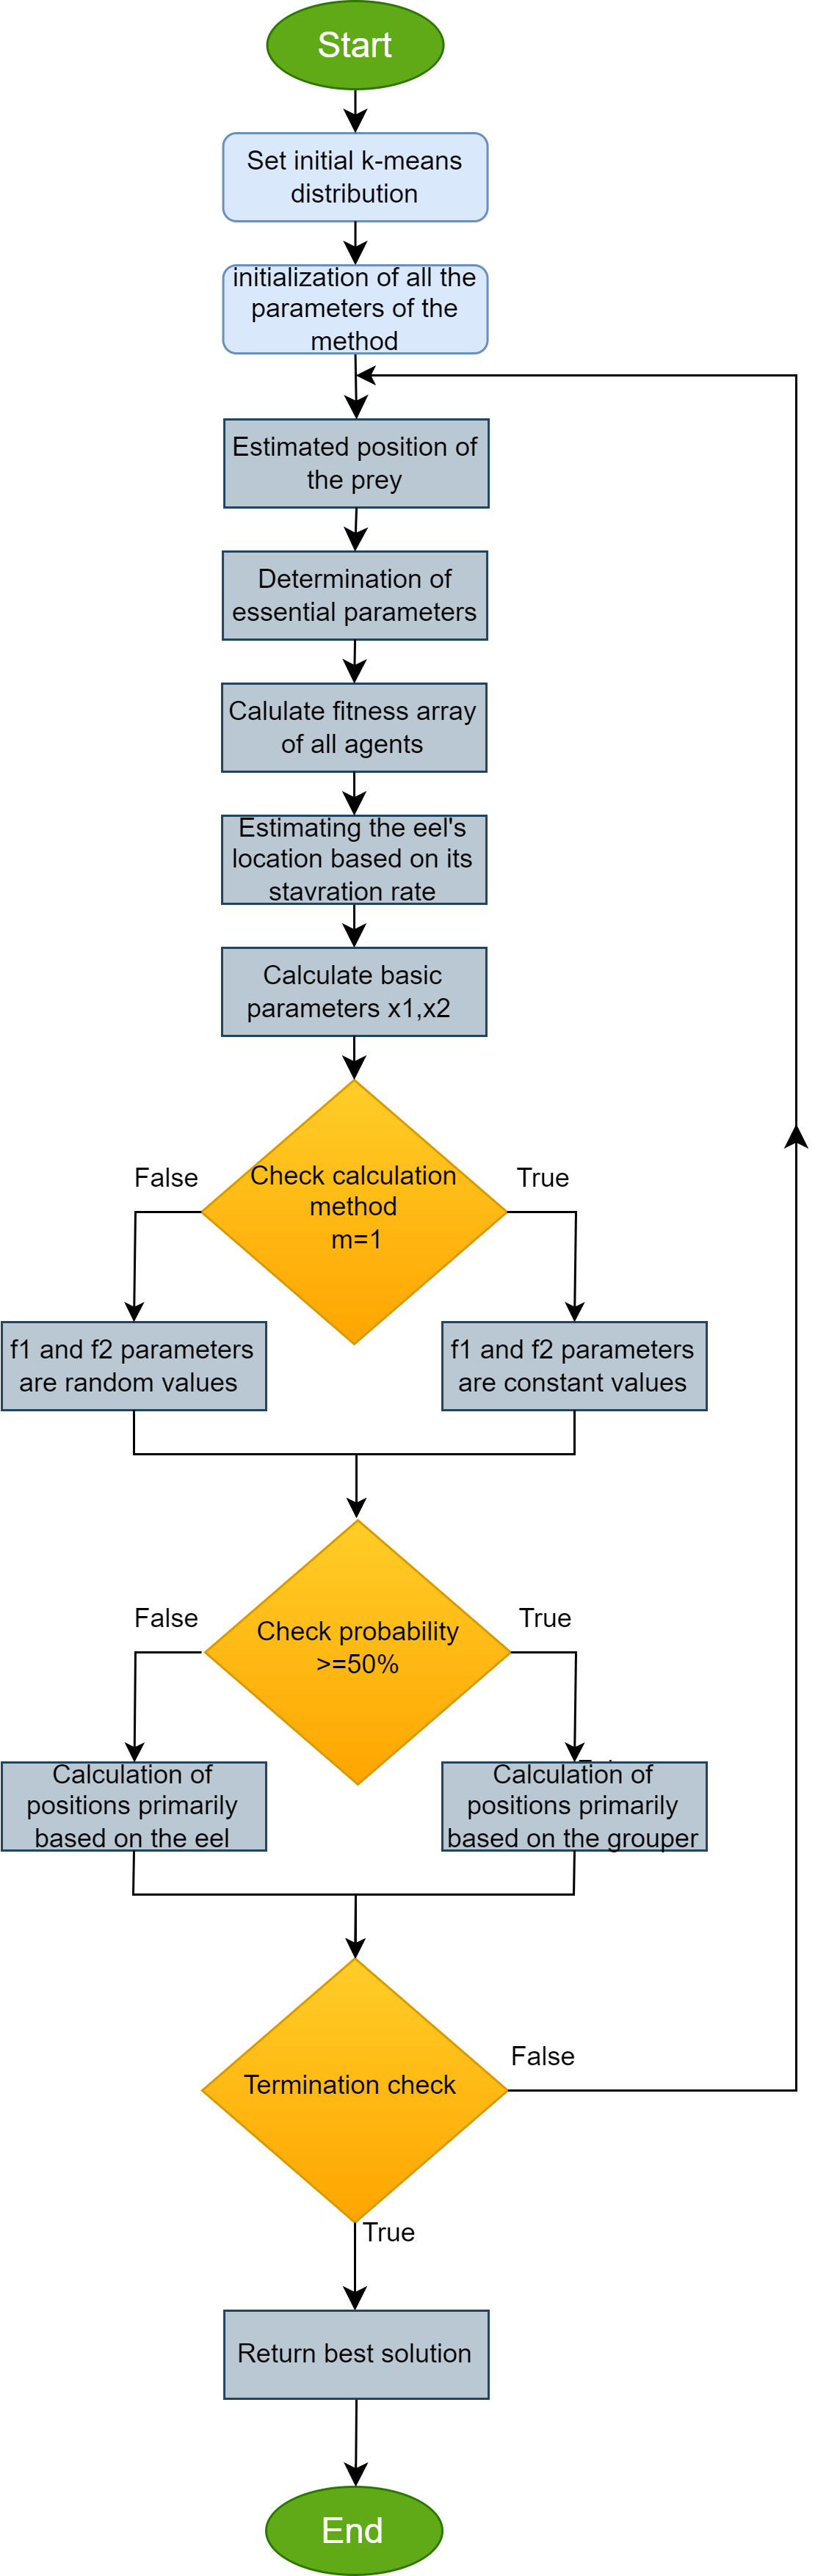
\includegraphics[scale=0.6]{eego.jpg}
\par\end{centering}
\caption{Flowchart of the suggested global optimization procedure.\label{fig:flowEgo}}

\end{figure}
The main modifications introduced by the proposed algorithm are the
following:
\begin{enumerate}
\item The members of the population are initialized using a procedure that
incorporates the K-means algorithm. This procedure is fully described
in subsection \ref{subsec:The-proposed-sampling}. The purpose of
this sampling technique is to produce points that are close to the
local minima of the objective problem through systematic clustering.
This will potentially significantly reduce the time required to complete
the technique. The samples used in the proposed algorithm are the
calculated centers of the K-means algorithm. This sampling technique
has been also utilized in some recent papers related to Global Optimization
techniques, such as the extended version of the Optimal Foraging algorithm
\citep{eofa} or the new Genetic Algorithm proposed by Charilogis
et al \citep{newGA}.
\item The second modification proposed is the stopping rule invoked at every
step of the algorithm. This rule measures the similarity between the
best fitness values obtained between consecutive iterations of the
algorithm. If this difference takes low values for a consecutive number
of iterations, then the algorithm may not be able to find a lower
value for the global minimum and should stop. This stopping rule have
been applied in the recent years in various methods such as in the
work of Charilogis and Tsoulos that presented an improved parallel
PSO method \citep{ppso}, the work of Kyrou at al. suggested an improved
version of the Giant - Armadillo optimization method \citep{igao}
or the recent work of Kyrou et al. that proposed an extended version
of the Optimal Foraging Algorithm \citep{eofa}. Of course, this method
is general enough for application in any global optimization procedure.
\item The third modification is the $m$ flag, which controls the randomness
in the range of candidate solutions. When this value is set to 2,
then the critical parameters $f_{1},f_{2}$ are calculated using random
numbers. 
\end{enumerate}
The overall procedure that outlines the basic steps of the method
and the added modifications is shown in Algorithm \ref{alg:The-basic-steps}.

\begin{algorithm}
\begin{enumerate}
\item \textbf{Initialize} the population members using a procedure incorporating
the K-means algorithm, shown in subsection \ref{subsec:The-proposed-sampling}
\item \textbf{Compute} the fitness of each search agent \label{enu:Compute-the-fitness}
\item \textbf{Sort} all solutions according to their fitness
\item \textbf{Calculate} the similarity stopping rule proposed in \citep{charilogis}
\end{enumerate}
\begin{itemize}
\item \textbf{If} the termination criteria are not satisfied then go to
step \ref{enu:Compute-the-fitness}
\item \textbf{else} terminate and return the best solution
\item \textbf{end if}
\end{itemize}
\caption{The basic steps of the algorithm accompanied with the proposed modifications.\label{alg:The-basic-steps}}

\end{algorithm}


\subsection{The used sampling procedure\label{subsec:The-proposed-sampling}}

The used sampling procedure that was incorporated in this work initially
generates samples from the objective problem. Then, using the K-means
method, only the estimated centers are selected as samples for the
proposed algorithm. This technique, which is an achievement of James
MacQueen \citep{MacQueen}, is one of the most well-known clustering
algorithms in the broad research community, both in data analysis
and in machine learning \citep{kmeans1-1} and pattern recognition
\citep{kmeans-paterrn}. The algorithm aims to divide a data set into
k clusters. The K-means algorithm tries to divide the data into groups
in such a way that the internal points of each group are as close
as possible to each other. At the same time, he tries to place the
central points of each group in positions which are as representative
as possible for the points of their group. During the past years a
series of variants of this algorithm has been proposed, such as the
Genetic K-means algotithm \citep{gen_kmeans}, the unsupervised K-means
algorithm \citep{unsuper_kmeans}, the Fixed-centered K-means algorithm
\citep{fixed_kmeans} etc. A review of K-Means clustering algorithms
can be found in the work of Oti et al. \citep{kmeans_review} Next,
the basic steps of the algorithm are provided in Algorithm \ref{alg:K-means-Algorithm}.
A flowchart of the K-Means procedure is also depicted in Figure \ref{fig:flowchartKmeans}.

\begin{algorithm}[H]
\begin{enumerate}
\item \textbf{Initialization}
\begin{enumerate}
\item \textbf{Set} $k$ the number of clusters.
\item \textbf{Obtain} randomly the initial samples $x_{i},\ i=1,\ldots,N_{m}$
\item \textbf{Set} $S=_{j}\{\ \}$, from $j=1,\ldots,k$.
\end{enumerate}
\item Repeat
\begin{enumerate}
\item \textbf{For} every point $x_{i},\ i=1,...,N_{m}$ \textbf{do}
\begin{enumerate}
\item \textbf{Set} $j^{*}=\mbox{argmin}_{m=1}^{k}\left\{ D\left(x_{i},c_{m}\right)\right\} $.
$j^{*}$ is the nearest center from $x_{i}$
\item \textbf{Set} $S_{j^{*}}=S_{j^{*}}\cup\left\{ x_{i}\right\} $.
\end{enumerate}
\item \textbf{End For}
\item \textbf{For} every center $c_{j},\ j=1..k$ \textbf{do}
\begin{enumerate}
\item \textbf{Set} $M_{j}$ the number of samples in $S_{j}$
\item \textbf{Update }the center $c_{j}$ as
\[
c_{j}=\frac{1}{M_{j}}\sum_{x_{i}\in S_{j}}x_{i}
\]
\end{enumerate}
\item \textbf{End} For
\end{enumerate}
\item Terminate when $c_{j}$ no longer changes
\item The final samples of the algorithm are the centers $c_{j}$.
\end{enumerate}
\caption{K-means Algorithm\label{alg:K-means-Algorithm}}
\end{algorithm}

\begin{figure}[H]
\begin{centering}
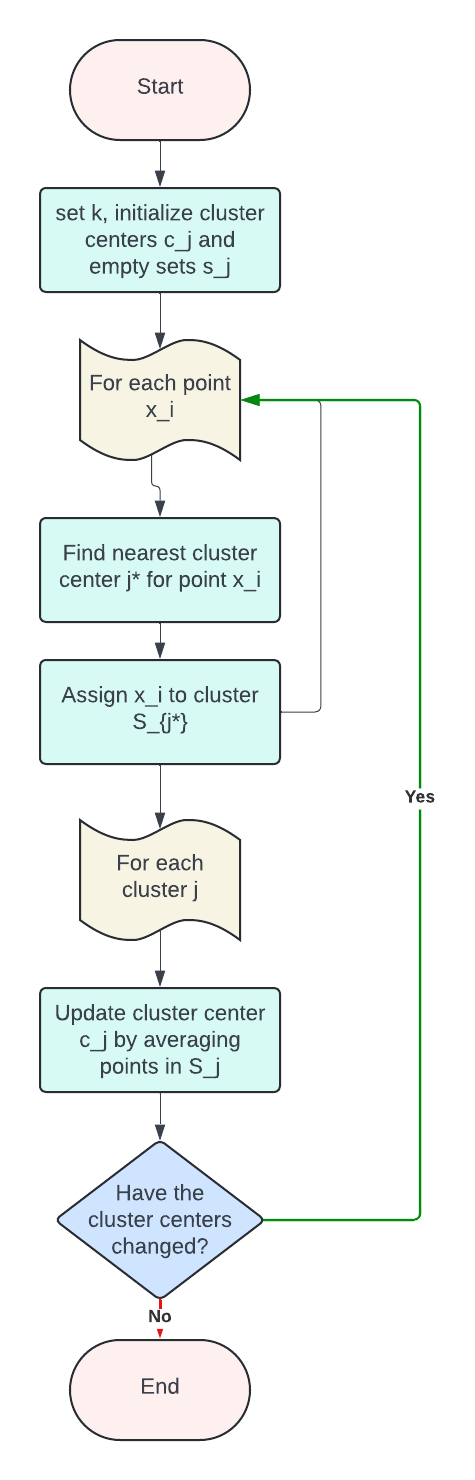
\includegraphics[scale=0.55]{kmeans_flowchart}
\par\end{centering}
\caption{The flowchart of the K-Means procedure.\label{fig:flowchartKmeans}}

\end{figure}


\section{Results\label{sec:Results}}

This section will begin with a detailed description of the functions
that will be used in the experiments, followed by an analysis of the
experiments performed and comparisons with other global optimization
techniques. 

\subsection{Test functions }

The test functions used in the experiments have been suggested in
a series of relative works \citep{Ali,Floudas1} and they originated
in a series of scientific fields. Also, these objective functions
have been studied in various publications \citep{testfunc1,testfunc2,testfunc2-1,testfunc3,testfunc4}.
Also, a series of function founded in \citep{gec} are used as test
functions. The used functions are defined as follows:
\begin{itemize}
\item \textbf{Ackley }function:
\[
f(x)=-a\exp\left(-b\sqrt{\frac{1}{n}\sum_{i=1}^{n}x_{i}^{2}}\right)-\exp\left(\frac{1}{n}\sum_{i=1}^{n}\cos\left(cx_{i}\right)\right)+a+\exp(1)
\]
with a=20.0.
\item \textbf{Bf1} (Bohachevsky 1) function:
\end{itemize}
\[
f(x)=x_{1}^{2}+2x_{2}^{2}-\frac{3}{10}\cos\left(3\pi x_{1}\right)-\frac{4}{10}\cos\left(4\pi x_{2}\right)+\frac{7}{10}
\]

\begin{itemize}
\item \textbf{Bf2} (Bohachevsky 2) function: 
\[
f(x)=x_{1}^{2}+2x_{2}^{2}-\frac{3}{10}\cos\left(3\pi x_{1}\right)\cos\left(4\pi x_{2}\right)+\frac{3}{10}
\]
\item \textbf{Bf3} (Bohachevsky 3) function: 
\[
f(x)=x_{1}^{2}+2x_{2}^{2}-\frac{3}{10}\cos\left(3\pi x_{1}+4\pi x_{2}\right)+\frac{3}{10}
\]
\item \textbf{Branin} function:

\[
f(x)=\left(x_{2}-\frac{5.1}{4\pi^{2}}x_{1}^{2}+\frac{5}{\pi}x_{1}-6\right)^{2}+10\left(1-\frac{1}{8\pi}\right)\cos(x_{1})+10
\]
 with $-5\le x_{1}\le10,\ 0\le x_{2}\le15$.
\item \textbf{Camel} function:
\[
f(x)=4x_{1}^{2}-2.1x_{1}^{4}+\frac{1}{3}x_{1}^{6}+x_{1}x_{2}-4x_{2}^{2}+4x_{2}^{4},\quad x\in[-5,5]^{2}
\]
\item \textbf{Easom} function: 
\[
f(x)=-\cos\left(x_{1}\right)\cos\left(x_{2}\right)\exp\left(\left(x_{2}-\pi\right)^{2}-\left(x_{1}-\pi\right)^{2}\right)
\]
with $x\in[-100,100]^{2}.$ 
\item \textbf{Equal maxima }function, defined as:
\[
f(x)=\sin^{6}\left(5\pi x\right)
\]
\item \textbf{Exponential} function, with the following definition: 
\[
f(x)=-\exp\left(-0.5\sum_{i=1}^{n}x_{i}^{2}\right),\quad-1\le x_{i}\le1
\]
The values $n=4,8,16,32$ were used in the conducted experiments.
\item \textbf{F9} test function:
\[
f(x)=-\sum_{i=1}^{n}\left(10+9\cos\left(2\pi k_{i}x_{i}\right)\right)
\]
with $x\in[0,1]^{n}.$
\item \textbf{Extended F10 }function:
\[
f(x)=\sum_{i=1}^{n}\left(x_{i}^{2}-10\cos\left(2\pi x_{i}\right)\right)
\]
\item \textbf{F14 }function:
\[
f(x)=\left(\frac{1}{500}+\sum_{j=1}^{25}\frac{1}{j+\sum_{i=1}^{2}\left(x_{i}-a_{ij}\right)^{6}}\right)^{-1}
\]
\item \textbf{F15 }function:
\[
f(x)=\sum_{i=1}^{11}\left(a_{i}-\frac{x_{1}\left(b_{i}+b_{i}x_{2}\right)}{b_{i}^{2}+b_{i}x_{3}+x_{4}}\right)^{2}
\]
\item \textbf{F17 }function:
\begin{align*}
f(x) & =\left(1+\left(x_{1}+x_{2}+1\right)^{2}\times\left(19-14x_{1}+3x_{1}^{2}-14x_{2}+6x_{1}x_{2}+3x_{2}^{2}\right)\right)\times\\
 & \left(30+\left(2x_{1}-3x_{2}\right)^{2}\times\left(18-32x_{1}+12x_{1}^{2}+48x_{2}-36x_{1}x_{2}+27x_{2}^{2}\right)\right)
\end{align*}
\item \textbf{Five - uneven - peak trap }function:
\[
f(x)=\begin{cases}
80(2.5-x) & 0\le x<2.5\\
64(x-2.5) & 2.5\le x<5.0\\
64(7.5-x) & 5.0\le x<7.5\\
28(x-7.5) & 7.5\le x<12.5\\
28(17.5-x) & 12.5\le x<17.5\\
32(x-17.5) & 17.5\le x<22.5\\
32(27.5-x) & 22.5\le x<27.5\\
80(x-27.5) & 27.5\le x\le30
\end{cases}
\]
\item \textbf{Himmelblau }function:
\[
f(x)=200-\left(x_{1}^{2}+x_{2}-11\right)^{2}-\left(x_{1}+x_{2}^{2}-7\right)^{2}
\]
with $x\in[-6,6]^{2}$.
\item \textbf{Griewank2} function:
\[
f(x)=1+\frac{1}{200}\sum_{i=1}^{2}x_{i}^{2}-\prod_{i=1}^{2}\frac{\cos(x_{i})}{\sqrt{(i)}},\quad x\in[-100,100]^{2}
\]
\item \textbf{Griewank10} function. The function is given by the equation
\[
f(x)=\sum_{i=1}^{n}\frac{x_{i}^{2}}{4000}-\prod_{i=1}^{n}\cos\left(\frac{x_{i}}{\sqrt{i}}\right)+1
\]
with $n=10$.
\item \textbf{Gkls} function \citep{gkls}. The function $f(x)=\mbox{Gkls}(x,n,w)$,
is a test function proposed in \citep{gkls} with $w$ local minima.
The values values $n=2,3$ and $w=50$ were used in the conducted
experiments.
\item \textbf{Goldstein and Price function }\\
\begin{eqnarray*}
f(x) & = & \left[1+\left(x_{1}+x_{2}+1\right)^{2}\right.\\
 &  & \left(19-14x_{1}+3x_{1}^{2}-14x_{2}+6x_{1}x_{2}+3x_{2}^{2}\right)]\times\\
 &  & [30+\left(2x_{1}-3x_{2}\right)^{2}\\
 &  & \left(18-32x_{1}+12x_{1}^{2}+48x_{2}-36x_{1}x_{2}+27x_{2}^{2}\right)]
\end{eqnarray*}
With $x\in[-2,2]^{2}$. 
\item \textbf{Hansen} function: $f(x)=\sum_{i=1}^{5}i\cos\left[(i-1)x_{1}+i\right]\sum_{j=1}^{5}j\cos\left[(j+1)x_{2}+j\right]$,
$x\in[-10,10]^{2}$ .
\item \textbf{Hartman 3} function:
\[
f(x)=-\sum_{i=1}^{4}c_{i}\exp\left(-\sum_{j=1}^{3}a_{ij}\left(x_{j}-p_{ij}\right)^{2}\right)
\]
with $x\in[0,1]^{3}$ and $a=\left(\begin{array}{ccc}
3 & 10 & 30\\
0.1 & 10 & 35\\
3 & 10 & 30\\
0.1 & 10 & 35
\end{array}\right),\ c=\left(\begin{array}{c}
1\\
1.2\\
3\\
3.2
\end{array}\right)$ and
\[
p=\left(\begin{array}{ccc}
0.3689 & 0.117 & 0.2673\\
0.4699 & 0.4387 & 0.747\\
0.1091 & 0.8732 & 0.5547\\
0.03815 & 0.5743 & 0.8828
\end{array}\right)
\]
\item \textbf{Hartman 6} function:
\[
f(x)=-\sum_{i=1}^{4}c_{i}\exp\left(-\sum_{j=1}^{6}a_{ij}\left(x_{j}-p_{ij}\right)^{2}\right)
\]
with $x\in[0,1]^{6}$ and $a=\left(\begin{array}{cccccc}
10 & 3 & 17 & 3.5 & 1.7 & 8\\
0.05 & 10 & 17 & 0.1 & 8 & 14\\
3 & 3.5 & 1.7 & 10 & 17 & 8\\
17 & 8 & 0.05 & 10 & 0.1 & 14
\end{array}\right),\ c=\left(\begin{array}{c}
1\\
1.2\\
3\\
3.2
\end{array}\right)$ and
\[
p=\left(\begin{array}{cccccc}
0.1312 & 0.1696 & 0.5569 & 0.0124 & 0.8283 & 0.5886\\
0.2329 & 0.4135 & 0.8307 & 0.3736 & 0.1004 & 0.9991\\
0.2348 & 0.1451 & 0.3522 & 0.2883 & 0.3047 & 0.6650\\
0.4047 & 0.8828 & 0.8732 & 0.5743 & 0.1091 & 0.0381
\end{array}\right)
\]
\item \textbf{Potential} function, this function represents the energy of
a molecular conformation of N atoms. The interaction of these atoms
is determined by the Lennard-Jones potential \citep{jones}. The definition
of this potential is:
\[
V_{LJ}(r)=4\epsilon\left[\left(\frac{\sigma}{r}\right)^{12}-\left(\frac{\sigma}{r}\right)^{6}\right]
\]
For the conducted experiments the values $N=3,\ 5$ were used. 
\item \textbf{Rastrigin} function. 
\[
f(x)=x_{1}^{2}+x_{2}^{2}-\cos(18x_{1})-\cos(18x_{2}),\quad x\in[-1,1]^{2}
\]
\item \textbf{\emph{Rosenbrock}}\emph{ function}.\\
\[
f(x)=\sum_{i=1}^{n-1}\left(100\left(x_{i+1}-x_{i}^{2}\right)^{2}+\left(x_{i}-1\right)^{2}\right),\quad-30\le x_{i}\le30.
\]
The values $n=4,\ 8,\ 16$ were incorporated in the conducted experiments.
\item \textbf{Shekel 5 }function.
\end{itemize}
\[
f(x)=-\sum_{i=1}^{5}\frac{1}{(x-a_{i})(x-a_{i})^{T}+c_{i}}
\]
 

with $x\in[0,10]^{4}$ and $a=\left(\begin{array}{cccc}
4 & 4 & 4 & 4\\
1 & 1 & 1 & 1\\
8 & 8 & 8 & 8\\
6 & 6 & 6 & 6\\
3 & 7 & 3 & 7
\end{array}\right),\ c=\left(\begin{array}{c}
0.1\\
0.2\\
0.2\\
0.4\\
0.4
\end{array}\right)$
\begin{itemize}
\item \textbf{Shekel 7} function.
\end{itemize}
\[
f(x)=-\sum_{i=1}^{7}\frac{1}{(x-a_{i})(x-a_{i})^{T}+c_{i}}
\]

with $x\in[0,10]^{4}$ and $a=\left(\begin{array}{cccc}
4 & 4 & 4 & 4\\
1 & 1 & 1 & 1\\
8 & 8 & 8 & 8\\
6 & 6 & 6 & 6\\
3 & 7 & 3 & 7\\
2 & 9 & 2 & 9\\
5 & 3 & 5 & 3
\end{array}\right),\ c=\left(\begin{array}{c}
0.1\\
0.2\\
0.2\\
0.4\\
0.4\\
0.6\\
0.3
\end{array}\right)$.
\begin{itemize}
\item \textbf{Shekel 10} function.
\end{itemize}
\[
f(x)=-\sum_{i=1}^{10}\frac{1}{(x-a_{i})(x-a_{i})^{T}+c_{i}}
\]
 

with $x\in[0,10]^{4}$ and $a=\left(\begin{array}{cccc}
4 & 4 & 4 & 4\\
1 & 1 & 1 & 1\\
8 & 8 & 8 & 8\\
6 & 6 & 6 & 6\\
3 & 7 & 3 & 7\\
2 & 9 & 2 & 9\\
5 & 5 & 3 & 3\\
8 & 1 & 8 & 1\\
6 & 2 & 6 & 2\\
7 & 3.6 & 7 & 3.6
\end{array}\right),\ c=\left(\begin{array}{c}
0.1\\
0.2\\
0.2\\
0.4\\
0.4\\
0.6\\
0.3\\
0.7\\
0.5\\
0.6
\end{array}\right)$. 
\begin{itemize}
\item \textbf{Sinusoidal} function defined as:
\[
f(x)=-\left(2.5\prod_{i=1}^{n}\sin\left(x_{i}-z\right)+\prod_{i=1}^{n}\sin\left(5\left(x_{i}-z\right)\right)\right),\quad0\le x_{i}\le\pi.
\]
The values $n=4,8,16$ were incorporated in the conducted experiments.
\item \textbf{Schaffer }function:\textbf{
\[
f(x)=\sum_{i=1}^{n}\left(\sum_{j=1}^{i}x_{j}\right)^{2}
\]
}
\item \textbf{Schwefel221 }function:
\[
f(x)=418.9829n+\sum_{i=1}^{n}-x_{i}\sin\left(\sqrt{\left|x_{i}\right|}\right)
\]
\item \textbf{Schwefel222} function:
\[
f(x)=\sum_{i=1}^{n}\left|x_{i}\right|+\prod_{i=1}^{n}\left|x_{i}\right|
\]
\item \textbf{Shubert }function:
\[
f(x)=-\prod_{i=1}^{n}\sum_{j=1}^{5}j\cos\left((j+1)x_{i}+j\right)
\]
with $x\in[-10,10]^{n}$
\item \textbf{Sphere }function:
\[
f(x)=\sum_{i=1}^{n}x_{i}^{2}
\]
\item \textbf{Test2N} function:
\[
f(x)=\frac{1}{2}\sum_{i=1}^{n}x_{i}^{4}-16x_{i}^{2}+5x_{i},\quad x_{i}\in[-5,5].
\]
The values $n=4,5,6,7$ were incorporated for the conducted experiments.
\item \textbf{Test30N} function:
\[
f(x)=\frac{1}{10}\sin^{2}\left(3\pi x_{1}\right)\sum_{i=2}^{n-1}\left(\left(x_{i}-1\right)^{2}\left(1+\sin^{2}\left(3\pi x_{i+1}\right)\right)\right)+\left(x_{n}-1\right)^{2}\left(1+\sin^{2}\left(2\pi x_{n}\right)\right)
\]
For the conducted experiments the values $n=3,4$ were used.
\item \textbf{Uneven decreasing maxima} function:
\[
f(x)=\exp\left(-2\log(2)\left(\frac{x-0.08}{0.854}\right)^{2}\right)\sin^{6}\left(5\pi\left(x^{\frac{3}{4}}-0.05\right)\right)
\]
\item \textbf{Vincent} function:
\[
f(x)=\frac{1}{n}\sum_{i=1}^{n}\sin\left(10\log\left(x_{i}\right)\right)
\]
with $x\in[0.25,10]^{n}$. 
\end{itemize}
%
Also, the dimension for each problem as used in the experiments is
shown in Table \ref{tab:functionDimension}.

\begin{table}[H]

\caption{The dimension for every function used in the experiments.\label{tab:functionDimension}}

\centering{}%
\begin{tabular}{|c|c|}
\hline 
FUNCTION & DIMENSION\tabularnewline
\hline 
\hline 
Ackley & $n=2$\tabularnewline
\hline 
Bf1 & $n=2$\tabularnewline
\hline 
Bf2 & $n=2$\tabularnewline
\hline 
Bf3 & $n=2$\tabularnewline
\hline 
Branin & $n=2$\tabularnewline
\hline 
Camel & $n=2$\tabularnewline
\hline 
Easom & $n=2$\tabularnewline
\hline 
EQUAL\_MAXIMA & $n=1$\tabularnewline
\hline 
EXP & $n=4,8,16,32$\tabularnewline
\hline 
EXTENDEDF10 & $n=2$\tabularnewline
\hline 
FIVE\_UNEVEN & $n=1$\tabularnewline
\hline 
F9 & $n=2$\tabularnewline
\hline 
F14 & $n=2$\tabularnewline
\hline 
F15 & $n=4$\tabularnewline
\hline 
F17 & $n=2$\tabularnewline
\hline 
HIMMELBLAU & $n=2$\tabularnewline
\hline 
GKLS & $n=2,3$\tabularnewline
\hline 
GRIEWANK2 & $n=2$\tabularnewline
\hline 
GRIEWANK10 & $n=10$\tabularnewline
\hline 
HANSEN & $n=2$\tabularnewline
\hline 
HARTMAN3 & $n=3$\tabularnewline
\hline 
HARTMAN6 & $n=6$\tabularnewline
\hline 
POTENTIAL & $n=9,15$\tabularnewline
\hline 
RASTRIGIN & $n=2$\tabularnewline
\hline 
ROSENBROCK & $n=4,8,16$\tabularnewline
\hline 
SHEKEL5 & $n=4$\tabularnewline
\hline 
SHEKEL7 & $n=4$\tabularnewline
\hline 
SHEKEL10 & $n=4$\tabularnewline
\hline 
SHUBERT & $n=2,4,8$\tabularnewline
\hline 
SCHWEFEL221 & $n=2$\tabularnewline
\hline 
SCHWEFEL222 & $n=2$\tabularnewline
\hline 
SPHERE & $n=2$\tabularnewline
\hline 
TEST2N & $n=4,5,6,7$\tabularnewline
\hline 
SINU & $n=4,8,16$\tabularnewline
\hline 
TEST30N & $n=3,4$\tabularnewline
\hline 
UNEVEN\_MAXIMA & $n=1$\tabularnewline
\hline 
VINCENT & $n=2,4,8$\tabularnewline
\hline 
\end{tabular}
\end{table}


\subsection{Experimental results}

A series of global optimization methods were applied to the mentioned
test functions. All experiments were performed 30 times using different
seed for the random generator and the average value of function calls
was measured. The used software was coded in ANSI C++ using the freely
available OPTIMUS optimization environment, that is available from
\url{https://github.com/itsoulos/OPTIMUS} (accessed on 27 September
2024). The experiments were executed on a Debian Linux system that
runs on an AMD Ryzen 5950X processor, with 128GB of RAM. In all cases
the BFGS \citep{powell} local optimization method was used at the
end of each global optimization technique to ensure that an actual
minimum will be discovered by the global optimization method. The
values for all experimental parameters are shown in Table \ref{tab:settings}.

\begin{table}[H]
\caption{The values used for every parameter of the used algorithms.}
\label{tab:settings}

\begin{tabular*}{1\textwidth}{@{\extracolsep{\fill}}>{\centering}p{0.33\textwidth}>{\centering}p{0.33\textwidth}>{\centering}p{0.33\textwidth}}
\toprule 
\textbf{PARAMETER} & \textbf{MEANING} & \textbf{VALUE}\tabularnewline
\midrule 
$N_{c}$ & Number of chromosomes/particles & 200\tabularnewline
\midrule 
$N_{g}$ & Maximum number of allowed iterations & 200\tabularnewline
\midrule 
$N_{m}$ & Number of samples for the K-means & $10\times N_{c}$\tabularnewline
\midrule
$N_{k}$ & Number of maximum iterations for stopping rule & 5\tabularnewline
\midrule
$p_{s}$ & Selection rate of the genetic algorithm & 0.1\tabularnewline
\midrule
$p_{m}$ & Mutation rate of the genetic algorithm & 0.05\tabularnewline
\bottomrule
\end{tabular*}
\end{table}
The experimental results for the test functions and a series of optimization
methods are shown in Table \ref{tab:comparison}, where the following
applies to this table:
\begin{itemize}
\item The column FUNCTION represents the used test function.
\item The column GENETIC represents the usage of a genetic algorithm \citep{genetic1,genetic2}
to the test function. This genetic algorithm is equipped with $N_{c}$
chromosomes and the maximum number of generations is set to $N_{g}$.
The modified version of Tsoulos \citep{doublepop} was used as a genetic
algorithm here.
\item The column PSO represents the incorporation of a Particle Swarm Optimizer
\citep{pso1,pso2} to each test function. This algorithm has $N_{c}$
particles and the maximum number of allowed iterations is set to $N_{g}$.
For the conducted experiments, the improved PSO method as proposed
by Charilogis and Tsoulos was used \citep{ipso}. 
\item The column DE\textbf{ }refers to the Differential Evolution method
\citep{diffe1,diffe2}.
\item The column EGO represents the initial method without the modifications
suggested in this work.
\item The column EEGO represents the usage of the proposed method. The corresponding
settings are shown in Table \ref{tab:settings}.
\item The row SUM is used to measure the total function calls for all problems.
\item If a method fails to find the global minimum over all runs this is
noted in the corresponding table with a percentage enclosed in parentheses
next to the average function calls. 
\end{itemize}
\begin{table}[H]
\caption{Experimental results using the incorporated optimization methods.
The numbers in parentheses denote standard deviation for the number
of function calls.\label{tab:comparison}}

\raggedright{}{\footnotesize{}}%
\begin{tabular}{|c|c|c|c|c|c|}
\hline 
\textbf{\tiny{}FUNCTION} & \textbf{\footnotesize{}GENETIC} & \textbf{\footnotesize{}PSO} & \textbf{\footnotesize{}DE} & \textbf{\footnotesize{}EGO} & \textbf{\footnotesize{}EEGO}\tabularnewline
\hline 
\hline 
{\tiny{}ACKLEY} & {\footnotesize{}6749 (869)} & {\footnotesize{}6885 (1108)} & {\footnotesize{}10220 (1342)} & {\footnotesize{}8714 (1009)} & \textbf{\footnotesize{}4199 (768)}\tabularnewline
\hline 
{\tiny{}BF1} & {\footnotesize{}4007 (308)} & {\footnotesize{}4142 (397)} & {\footnotesize{}8268 (299)} & {\footnotesize{}4762 (379)} & \textbf{\footnotesize{}3228 (356)}\tabularnewline
\hline 
{\tiny{}BF2} & {\footnotesize{}3794 (350)} & {\footnotesize{}3752 (302)} & {\footnotesize{}7913 (320)} & {\footnotesize{}4299 (325)} & \textbf{\footnotesize{}2815 (310)}\tabularnewline
\hline 
{\tiny{}BF3} & {\footnotesize{}3480 (266)} & {\footnotesize{}3306 (261)} & {\footnotesize{}10270 (294)} & {\footnotesize{}3747 (303)} & \textbf{\footnotesize{}2501 (218)}\tabularnewline
\hline 
{\tiny{}BRANIN} & {\footnotesize{}2376 (136)} & {\footnotesize{}2548 (142)} & {\footnotesize{}4101 (559)} & {\footnotesize{}2659 (150)} & \textbf{\footnotesize{}1684 (180)}\tabularnewline
\hline 
{\tiny{}CAMEL} & {\footnotesize{}2869 (195)} & {\footnotesize{}2933 (180)} & {\footnotesize{}5609 (530)} & {\footnotesize{}3317 (229)} & \textbf{\footnotesize{}2262 (295)}\tabularnewline
\hline 
{\tiny{}EASOM} & {\footnotesize{}1958 (67)} & {\footnotesize{}1982 (92)} & {\footnotesize{}2978 (344)} & {\footnotesize{}2235 (196)} & \textbf{\footnotesize{}1334 (133)}\tabularnewline
\hline 
{\tiny{}EQUAL\_MAXIMA} & {\footnotesize{}2651 (131)} & {\footnotesize{}1499 (176)} & {\footnotesize{}2374 (117)} & {\footnotesize{}2013 (157)} & \textbf{\footnotesize{}1286 (121)}\tabularnewline
\hline 
{\tiny{}EXP4} & {\footnotesize{}2946 (196)} & {\footnotesize{}3404 (201)} & {\footnotesize{}5166 (430)} & {\footnotesize{}3392 (313)} & \textbf{\footnotesize{}2166 (243)}\tabularnewline
\hline 
{\tiny{}EXP8} & {\footnotesize{}3120 (187)} & {\footnotesize{}3585 (212)} & {\footnotesize{}5895 (615)} & {\footnotesize{}3347 (288)} & \textbf{\footnotesize{}2802 (304)}\tabularnewline
\hline 
{\tiny{}EXP16} & \textbf{\footnotesize{}3250 (234)} & {\footnotesize{}3735 (206)} & {\footnotesize{}6498 (784)} & {\footnotesize{}3345 (233)} & {\footnotesize{}3279 (416)}\tabularnewline
\hline 
{\tiny{}EXP32} & {\footnotesize{}3561 (233)} & {\footnotesize{}3902 (233)} & {\footnotesize{}7606 (475)} & \textbf{\footnotesize{}3332 (250)} & {\footnotesize{}3430 (401)}\tabularnewline
\hline 
{\tiny{}EXTENDEDF10} & {\footnotesize{}4862 (959)} & {\footnotesize{}3653 (329)} & {\footnotesize{}5728 (976) (0.87)} & {\footnotesize{}4737 (428)} & \textbf{\footnotesize{}2609 (321)}\tabularnewline
\hline 
{\tiny{}FIVE\_UNEVEN} & \textbf{\footnotesize{}3412 (422) (0.67)} & {\footnotesize{}3913 (378)(0.87)} & {\footnotesize{}4042 (391) (0.14)} & {\footnotesize{}5006 (519) (0.97)} & {\footnotesize{}3849 (388)(0.90)}\tabularnewline
\hline 
{\tiny{}F9} & {\footnotesize{}2604 (197)} & {\footnotesize{}1888 (306)} & {\footnotesize{}2271 (364) } & {\footnotesize{}2748 (333)} & \textbf{\footnotesize{}1439 (229)}\tabularnewline
\hline 
{\tiny{}F14} & {\footnotesize{}6686 (1503)} & {\footnotesize{}5498 (550)} & \textbf{\footnotesize{}5279 (1988) (0.63)} & {\footnotesize{}9228 (3725) (0.94)} & {\footnotesize{}6063 (1835)}\tabularnewline
\hline 
{\tiny{}F15} & \textbf{\footnotesize{}4373 (624)} & {\footnotesize{}6696 (856)} & {\footnotesize{}5874 (1880) (0.80)} & {\footnotesize{}7342 (1441)} & {\footnotesize{}4397 (1031)}\tabularnewline
\hline 
{\tiny{}F17} & {\footnotesize{}3667 (267)} & {\footnotesize{}3805 (333)} & {\footnotesize{}10441 (1435)} & {\footnotesize{}4057 (339)} & \textbf{\footnotesize{}2766 (368)}\tabularnewline
\hline 
{\tiny{}HIMMELBLAU} & {\footnotesize{}2481 (27)} & \textbf{\footnotesize{}1013 (34)} & {\footnotesize{}6636 (282)} & {\footnotesize{}1718 (84)} & {\footnotesize{}1119 (81)}\tabularnewline
\hline 
{\tiny{}GKLS250} & {\footnotesize{}2280 (184)} & {\footnotesize{}2411 (158)} & {\footnotesize{}3834 (416)} & {\footnotesize{}3332 (203)} & {\footnotesize{}1603 (150)}\tabularnewline
\hline 
{\tiny{}GKLS350} & {\footnotesize{}2613 (269)} & {\footnotesize{}2234 (225)} & {\footnotesize{}3919 (469)} & {\footnotesize{}2493 (233)} & \textbf{\footnotesize{}1298 (178)}\tabularnewline
\hline 
{\tiny{}GOLDSTEIN} & {\footnotesize{}3687 (278)} & {\footnotesize{}3865 (356)} & {\footnotesize{}6781 (483)} & {\footnotesize{}4015 (323)} & \textbf{\footnotesize{}2784 (290)}\tabularnewline
\hline 
{\tiny{}GRIEWANK2} & {\footnotesize{}4501 (918)} & {\footnotesize{}3076 (218) (0.73)} & {\footnotesize{}7429 (1472)} & {\footnotesize{}4682 (586)} & \textbf{\footnotesize{}2589 (532) (0.96)}\tabularnewline
\hline 
{\tiny{}GRIEWANK10} & \textbf{\footnotesize{}6410 (1264) (0.97)} & {\footnotesize{}8006 (732)} & {\footnotesize{}18490 (1716)} & {\footnotesize{}8772 (1138)} & {\footnotesize{}7435 (900)}\tabularnewline
\hline 
{\tiny{}HANSEN} & {\footnotesize{}3210 (458)} & {\footnotesize{}2856 (208)} & {\footnotesize{}4185 (627)} & {\footnotesize{}3789 (864)} & \textbf{\footnotesize{}2484 (417)}\tabularnewline
\hline 
{\tiny{}HARTMAN3} & {\footnotesize{}2752 (188)} & {\footnotesize{}3140 (215)} & {\footnotesize{}5190 (294)} & {\footnotesize{}3078 (267)} & \textbf{\footnotesize{}1793 (231)}\tabularnewline
\hline 
{\tiny{}HARTMAN6} & {\footnotesize{}3219 (217)} & {\footnotesize{}3710 (235)} & {\footnotesize{}5968 (548)} & {\footnotesize{}3583 (309)} & \textbf{\footnotesize{}2478 (282)}\tabularnewline
\hline 
{\tiny{}POTENTIAL3} & {\footnotesize{}4352 (461)} & {\footnotesize{}4865 (468)} & {\footnotesize{}6118 (1047)} & {\footnotesize{}6027 (793)} & \textbf{\footnotesize{}4081 (391)}\tabularnewline
\hline 
{\tiny{}POTENTIAL5} & \textbf{\footnotesize{}7705 (892)} & {\footnotesize{}9183 (1180)} & {\footnotesize{}9119 (570)} & {\footnotesize{}9968 (1171)} & {\footnotesize{}8886 (1146)}\tabularnewline
\hline 
{\tiny{}RASTRIGIN} & {\footnotesize{}4107 (729)} & {\footnotesize{}3477 (348)} & {\footnotesize{}6216 (428)} & {\footnotesize{}4201 (401)} & \textbf{\footnotesize{}2304 (302)}\tabularnewline
\hline 
{\tiny{}ROSENBROCK4} & \textbf{\footnotesize{}3679 (393)} & {\footnotesize{}6372 (549)} & {\footnotesize{}8452 (643)} & {\footnotesize{}6137 (720)} & {\footnotesize{}4019 (324)}\tabularnewline
\hline 
{\tiny{}ROSENBROCK8} & \textbf{\footnotesize{}5270 (514)} & {\footnotesize{}8284 (849)} & {\footnotesize{}11530 (1632)} & {\footnotesize{}8569 (872)} & {\footnotesize{}6801 (633)}\tabularnewline
\hline 
{\tiny{}ROSENBROCK16} & \textbf{\footnotesize{}8509 (1026)} & {\footnotesize{}11872 (1018)} & {\footnotesize{}17432 (1738)} & {\footnotesize{}11777 (1268)} & {\footnotesize{}11996 (1331)}\tabularnewline
\hline 
{\tiny{}SHEKEL5} & {\footnotesize{}3325 (227)} & {\footnotesize{}4259 (305)} & {\footnotesize{}6662 (974) } & {\footnotesize{}3948 (340)} & \textbf{\footnotesize{}2495 (310)}\tabularnewline
\hline 
{\tiny{}SHEKEL7} & {\footnotesize{}3360 (283)} & {\footnotesize{}4241 (300)} & {\footnotesize{}6967 (1035)} & {\footnotesize{}4043 (379)} & \textbf{\footnotesize{}2432 (240)}\tabularnewline
\hline 
{\tiny{}SHEKEL10} & {\footnotesize{}3488 (240)} & {\footnotesize{}4237 (268)} & {\footnotesize{}6757 (897)} & {\footnotesize{}3932 (355)} & \textbf{\footnotesize{}2516 (326)}\tabularnewline
\hline 
{\tiny{}SHUBERT2} & {\footnotesize{}3567 (413)} & \textbf{\footnotesize{}2123 (188)} & {\footnotesize{}3526 (885)} & {\footnotesize{}3622 (446)} & {\footnotesize{}2300 (527)}\tabularnewline
\hline 
{\tiny{}SHUBERT4} & {\footnotesize{}3358 (380)} & \textbf{\footnotesize{}1823 (166)} & {\footnotesize{}3067 (699)} & {\footnotesize{}3593 (674)} & {\footnotesize{}1967 (323) (0.97)}\tabularnewline
\hline 
{\tiny{}SHUBERT8} & {\footnotesize{}3569 (357)} & {\footnotesize{}2348 (203)} & {\footnotesize{}3120 (452) (0.94)} & {\footnotesize{}2862 (383)} & \textbf{\footnotesize{}2267 (296)}\tabularnewline
\hline 
{\tiny{}SCHAFFER} & {\footnotesize{}18787 (3105)} & {\footnotesize{}15176 (2401)} & \textbf{\footnotesize{}6315 (1548)} & {\footnotesize{}28679 (6267)} & {\footnotesize{}23531 (5904)}\tabularnewline
\hline 
{\tiny{}SCHWEFEL221} & {\footnotesize{}2667 (416)} & {\footnotesize{}2529 (163)} & {\footnotesize{}5415 (1161)} & {\footnotesize{}3426 (787)} & \textbf{\footnotesize{}2203 (478)}\tabularnewline
\hline 
{\tiny{}SCHWEFEL222} & {\footnotesize{}33725 (4809)} & {\footnotesize{}42898 (6978)} & \textbf{\footnotesize{}12200 (1737)} & {\footnotesize{}51654 (7150)} & {\footnotesize{}38876 (5659)}\tabularnewline
\hline 
{\tiny{}SPHERE} & {\footnotesize{}1588 (23)} & {\footnotesize{}1521 (12)} & {\footnotesize{}3503 (199)} & {\footnotesize{}1642 (38)} & \textbf{\footnotesize{}1162 (84)}\tabularnewline
\hline 
{\tiny{}TEST2N4} & {\footnotesize{}3331 (392)} & {\footnotesize{}3437 (223)} & {\footnotesize{}6396 (999)} & {\footnotesize{}3695 (411)} & \textbf{\footnotesize{}2277 (464)}\tabularnewline
\hline 
{\tiny{}TEST2N5} & {\footnotesize{}4000 (815)} & {\footnotesize{}3683 (287)} & {\footnotesize{}6271 (1017)} & {\footnotesize{}4234 (636)} & \textbf{\footnotesize{}2734 (479) (0.96)}\tabularnewline
\hline 
{\tiny{}TEST2N6} & {\footnotesize{}4312 (901) (0.93)} & {\footnotesize{}3781 (241)} & {\footnotesize{}5410 (822) (0.93)} & {\footnotesize{}4599 (589)} & \textbf{\footnotesize{}2905 (832) (0.86)}\tabularnewline
\hline 
{\tiny{}TEST2N7} & {\footnotesize{}4775 (905) (0.90)} & {\footnotesize{}4060 (312)} & {\footnotesize{}7074 (1523) (0.97)} & {\footnotesize{}5146 (767)} & \textbf{\footnotesize{}3559 (763) (0.73)}\tabularnewline
\hline 
{\tiny{}SINU4} & {\footnotesize{}2991 (298)} & {\footnotesize{}3504 (231)} & {\footnotesize{}5953 (1509)} & {\footnotesize{}3478 (463)} & \textbf{\footnotesize{}2005 (332)}\tabularnewline
\hline 
{\tiny{}SINU8} & {\footnotesize{}3442 (293)} & {\footnotesize{}4213 (309)} & {\footnotesize{}6973 (1637)} & {\footnotesize{}4420 (560)} & \textbf{\footnotesize{}3158 (467)}\tabularnewline
\hline 
{\tiny{}SINU16} & \textbf{\footnotesize{}4320 (458)} & {\footnotesize{}5019 (312)} & {\footnotesize{}6979 (634)} & {\footnotesize{}7033 (1017)} & {\footnotesize{}5891 (553)}\tabularnewline
\hline 
{\tiny{}TEST30N3} & {\footnotesize{}3211 (1207)} & {\footnotesize{}4610 (1615)} & {\footnotesize{}6168 (1297)} & {\footnotesize{}3971 (1348)} & \textbf{\footnotesize{}2362 (884)}\tabularnewline
\hline 
{\tiny{}TEST30N4} & {\footnotesize{}3679 (1435)} & {\footnotesize{}4629 (1708)} & {\footnotesize{}7006 (2745)} & {\footnotesize{}4908 (1333)} & \textbf{\footnotesize{}2978 (1719)}\tabularnewline
\hline 
{\tiny{}UNEVEN\_MAXIMA} & {\footnotesize{}2969 (283)} & {\footnotesize{}2729 (292)} & {\footnotesize{}2393 (319)} & {\footnotesize{}2972 (288)} & \textbf{\footnotesize{}1560 (208)}\tabularnewline
\hline 
{\tiny{}VINCENT2} & {\footnotesize{}12779 (563)} & \textbf{\footnotesize{}1797 (140) (0.87)} & {\footnotesize{}6216 (1152)} & {\footnotesize{}2094 (148)} & {\footnotesize{}1834 (388) (0.90)}\tabularnewline
\hline 
{\tiny{}VINCENT4} & {\footnotesize{}19385 (1179)} & \textbf{\footnotesize{}1830 (190) (0.67)} & {\footnotesize{}4691 (1019) (0.83)} & {\footnotesize{}2674 (244)} & {\footnotesize{}2697 (1443) (0.64)}\tabularnewline
\hline 
{\tiny{}VINCENT8} & {\footnotesize{}19882 (2548)} & \textbf{\footnotesize{}2717 (256)} & {\footnotesize{}4417 (1118) (0.77)} & {\footnotesize{}3423 (358)} & {\footnotesize{}4368 (2253) (0.77)}\tabularnewline
\hline 
\textbf{\tiny{}SUM} & \textbf{\footnotesize{}297650} & \textbf{\footnotesize{}268654} & \textbf{\footnotesize{}288413} & \textbf{\footnotesize{}320469} & \textbf{\footnotesize{}231856}\tabularnewline
\hline 
\end{tabular}{\footnotesize\par}
\end{table}
The same termination method, as detailed in subsection \ref{subsec:The-main-steps},
was used in all global optimization techniques in order to be able
to evaluate all techniques fairly and with the same rules. In figure
\ref{fig:TotalFunctionCalls} we present the total function calls
of every optimization method is presented graphically. The proposed
method has excellent results compared to the other optimization techniques
according to the experiment we conducted. As we can observe it has
the least number of calls than all the other techniques. 
\begin{figure}[H]
\centering{}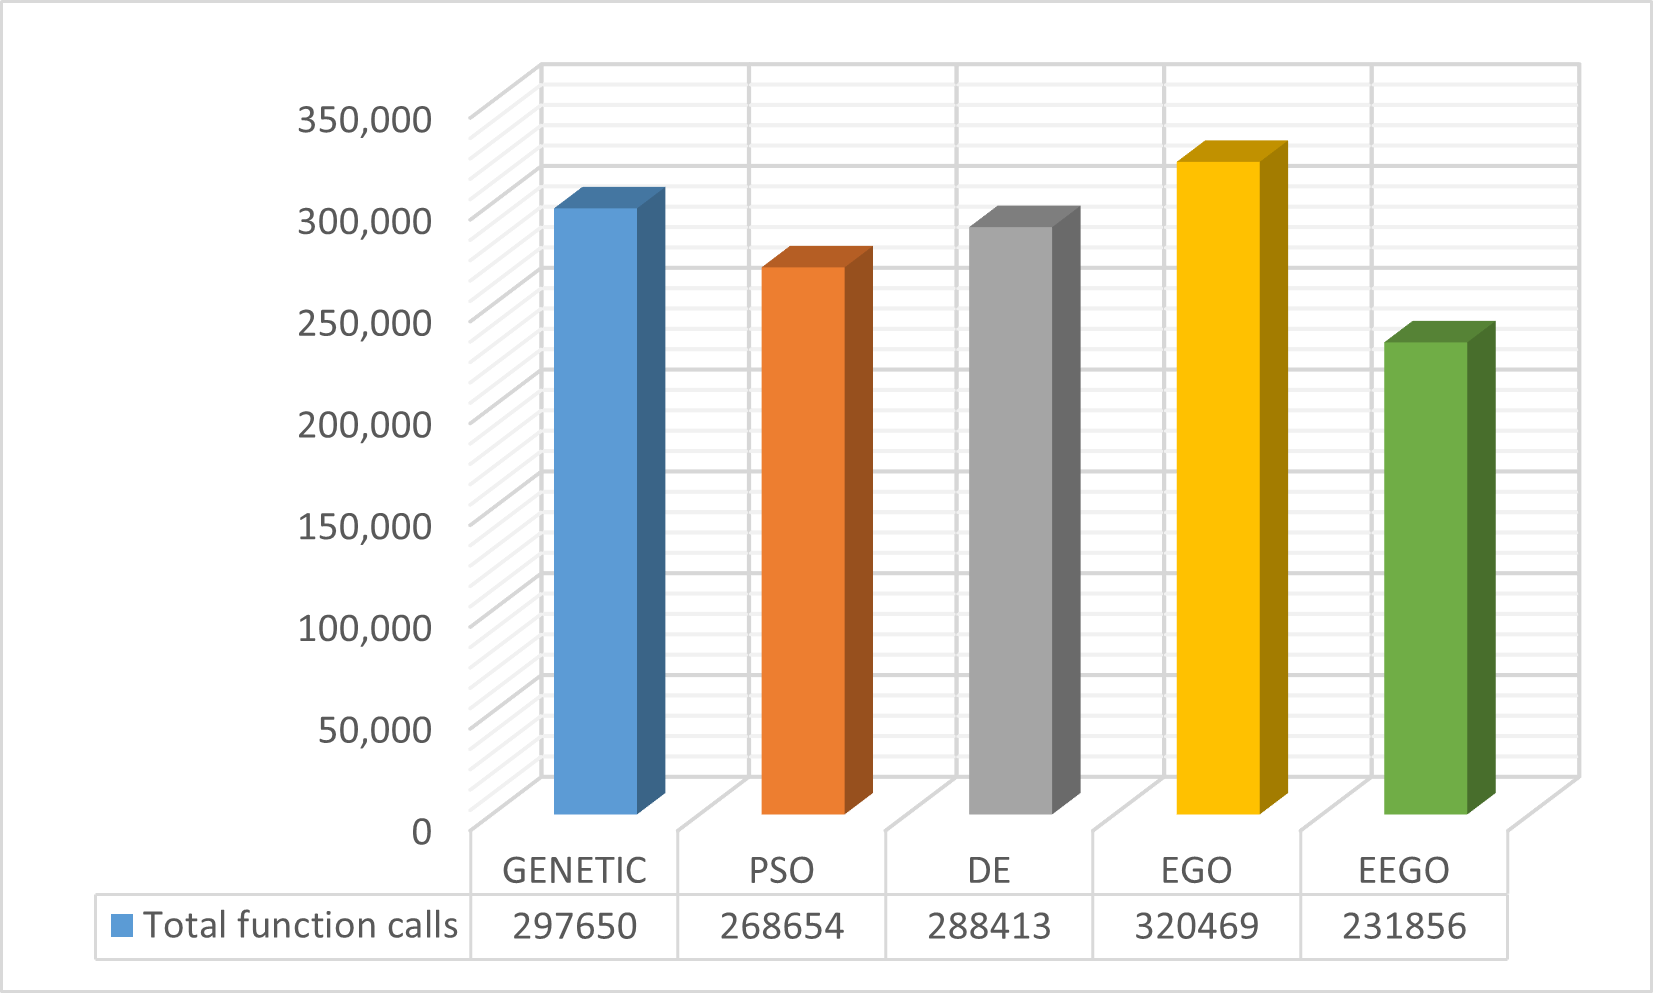
\includegraphics{image2}\caption{Total function calls for the incorporated optimization methods. The
numbers represent the sum of function calls for each mentioned method.\label{fig:TotalFunctionCalls}}
\end{figure}
. Furthermore, as the experimental results clearly indicate, the modified
version outperforms the original EGO method in terms of average and
function calls and this is depicted in Figure \ref{fig:boxPlotEgo}
that outlines box plots for the mentioned methods.
\begin{figure}[H]
\begin{centering}
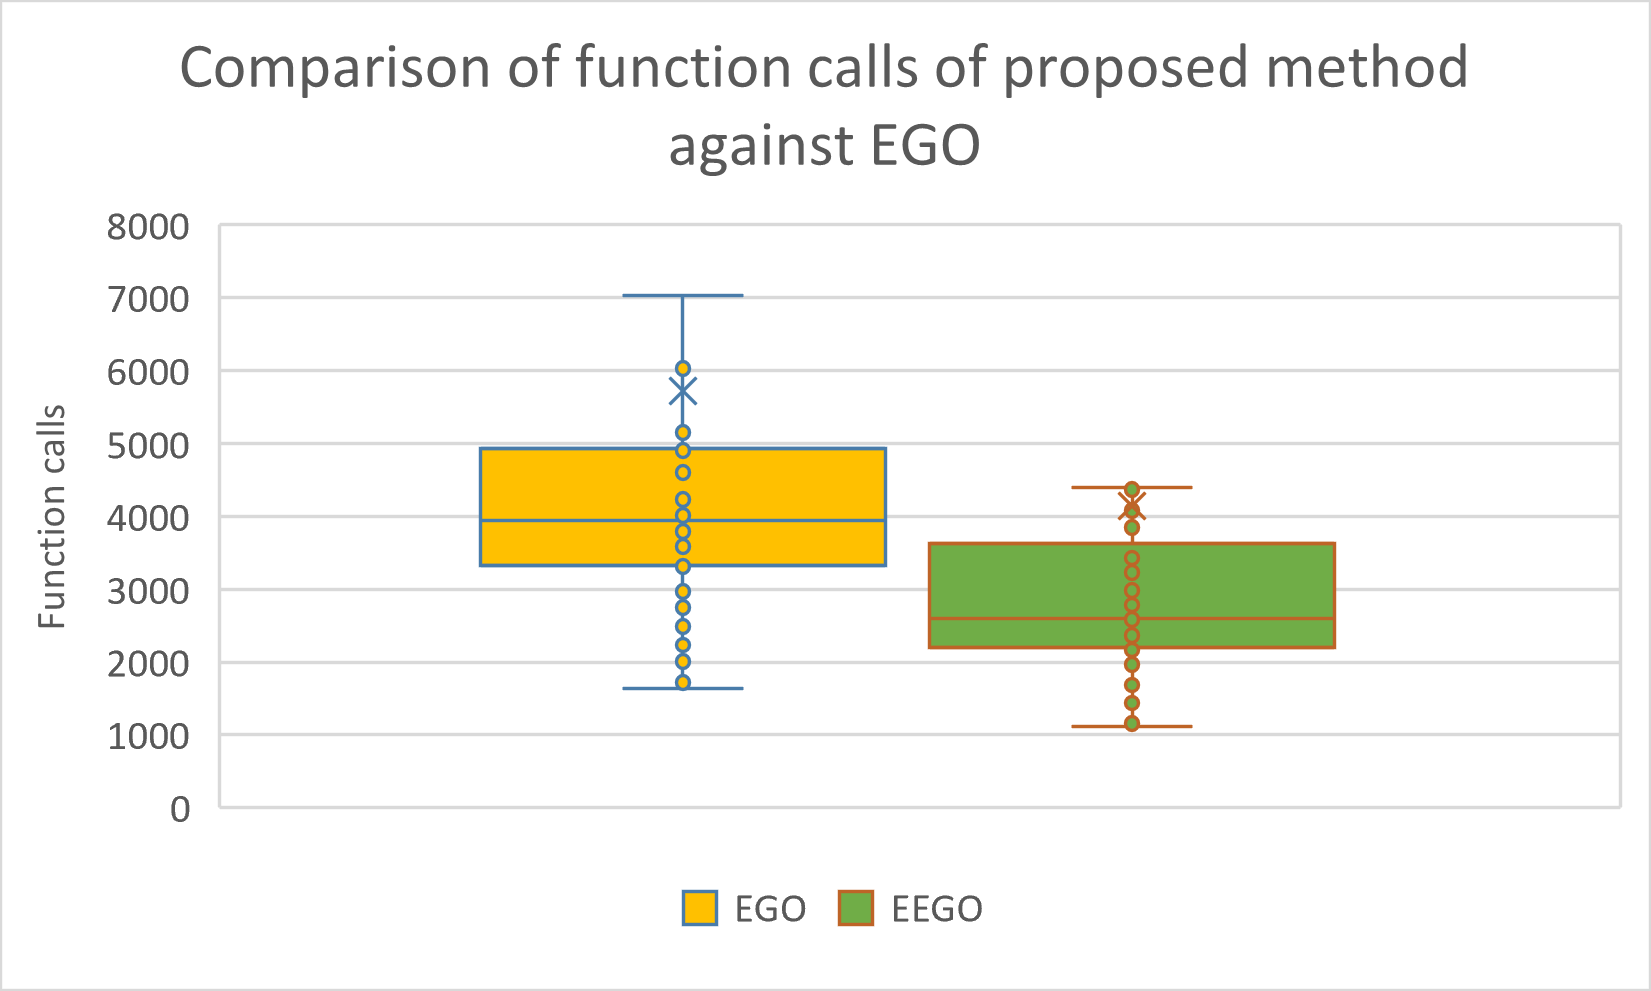
\includegraphics{boxego}
\par\end{centering}
\caption{Box plot used to compare the methods EGO and the modified version
as suggested in the current work.\label{fig:boxPlotEgo}}

\end{figure}
 A box plot between all the used methods is depicted in in Figure
\ref{fig:functionCalls}.
\begin{figure}[H]
\centering{}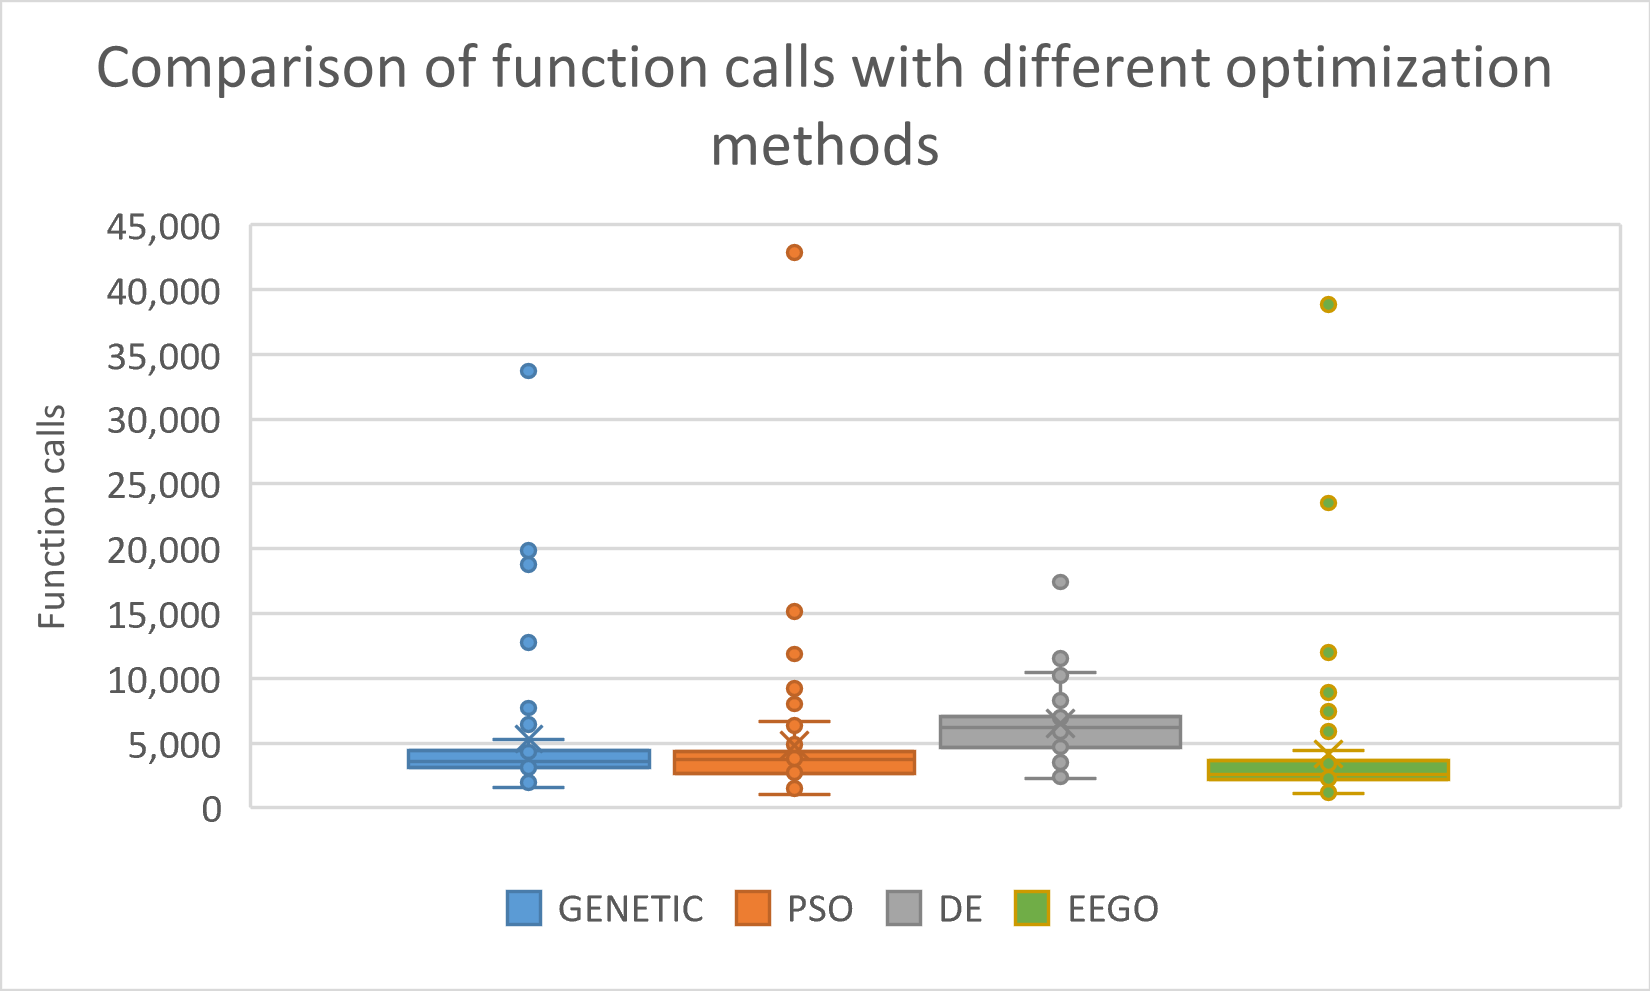
\includegraphics{image1}\caption{Comparison of average function calls for the incorporated optimization
methods, using proposed initial distribution\label{fig:functionCalls}}
\end{figure}
 Moreover, a statistical comparison for all used methods is outlined
in Figure \ref{fig:statAllMethods}.

\begin{figure}[H]
\begin{centering}
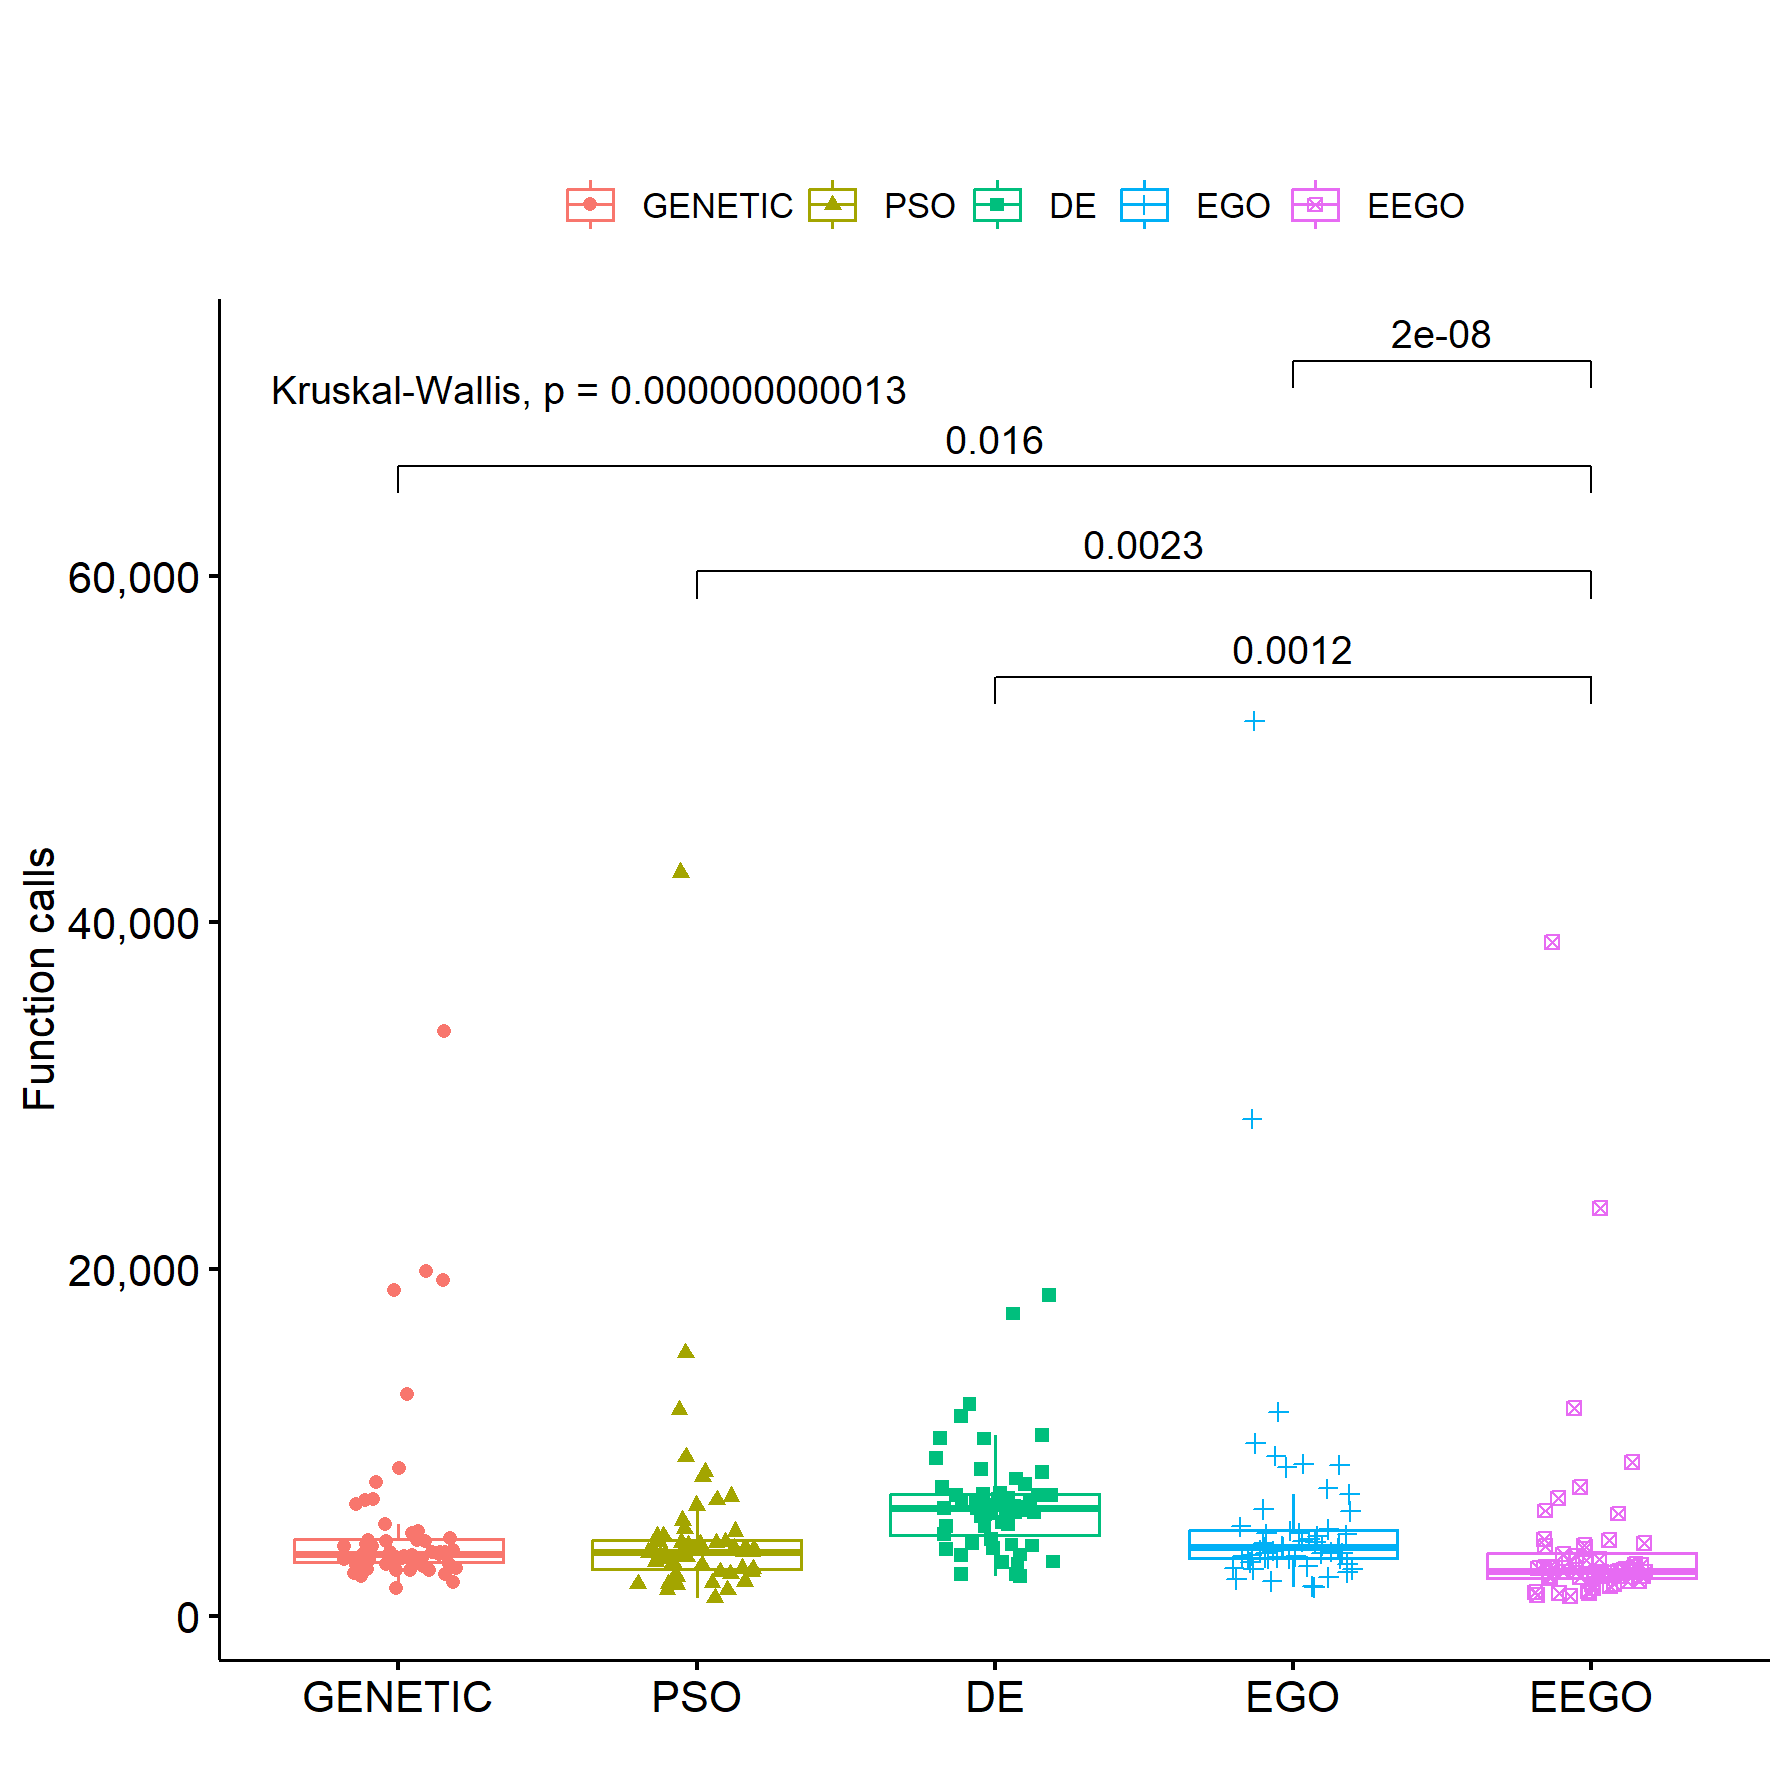
\includegraphics[scale=0.5]{Rplot}
\par\end{centering}
\caption{Statistical comparison of all used methods.\label{fig:statAllMethods}}

\end{figure}

According to Table \ref{tab:comparison} and Figure \ref{fig:statAllMethods},
the EEGO method proves to be more efficient, as it consistently requires
fewer function calls compared to the DE, PSO, GENETIC, and EGO methods,
and these differences are statistically significant (p \textless{}
0.05). For example, in the ACKLEY function, EEGO required 4199 calls,
while DE required 10.220, PSO 6885, and GENETIC 6749, with a p-value
\textless{} 0.05, showing that EEGO is significantly more efficient.
Similar examples are observed in the BF1 function, where EEGO had
3228 calls, while DE required 8268 (p \textless{} 0.05), and in the
BRANIN function, where EEGO required 1684 calls, compared to 4101
for DE (p \textless{} 0.05). Overall, EEGO shows the best performance
in most cases, with statistically significant differences in function
calls, as it effectively reduces the number of calls compared to the
other methods. While PSO and GENETIC perform better than DE in some
instances, they still lag significantly behind EEGO. The p-values
confirm that these differences are statistically significant, indicating
that EEGO is the most efficient method overall.

One more experiment which was performed with the ultimate goal of
measuring the importance of K-means sampling in the proposed method.
The results for this experiment are outlined in Table \ref{tab:sampling}
and the following sampling methods were used:
\begin{enumerate}
\item The column UNIFORM represents the usage of uniform sampling in the
current method.
\item The column TRIANGULAR stands for the usage of the triangular distribution
\citep{triangular} for sampling.
\item The column MAXWELL represents for the application of the Maxwell distribution
\citep{maxwell} to produce initial samples for the used method.
\item The column KMEANS represents the usage of the method described in
subsection \ref{subsec:The-proposed-sampling} to produce initial
samples for the used method.
\end{enumerate}
\begin{table}[H]
\caption{A series of sampling techniques is used in the proposed method.  The
numbers in parentheses denote standard deviation for the number of
function calls. \label{tab:sampling}}

\centering{}%
\begin{tabular}{|c|c|c|c|c|}
\hline 
\textbf{FUNCTION} & \textbf{UNIFORM} & \textbf{TRIANGULAR} & \textbf{MAXWELL} & \textbf{KMEANS}\tabularnewline
\hline 
\hline 
ACKLEY & 6118 (736) & 5912 (741) & 5986 (845) & \textbf{4199 (768)}\tabularnewline
\hline 
BF1 & 4513 (423) & 4318 (368) & 4055 (346) & \textbf{3228 (356)}\tabularnewline
\hline 
BF2 & 3959 (333) & 3879 (363) & 3587 (339) & \textbf{2815 (310)}\tabularnewline
\hline 
BF3 & 3506 (286) & 3344 (254) & 3129 (298) & \textbf{2501 (218)}\tabularnewline
\hline 
BRANIN & 2282 (162) & 2131 (174) & 2066 (167) & \textbf{1684 (180)}\tabularnewline
\hline 
CAMEL & 3156 (251) & 2919 (244) & 2848 (261) & \textbf{2262 (295)}\tabularnewline
\hline 
EASOM & 1756 (138) & 1650 (140) & \textbf{1321 (106)} & 1334 (133)\tabularnewline
\hline 
EQUAL\_MAXIMA & 1445 (130) & 1293 (115) & \textbf{1165 (139)} & 1286 (121)\tabularnewline
\hline 
EXP4 & 3438 (335) & 3273 (232) & 3194 (330) & \textbf{2166 (243)}\tabularnewline
\hline 
EXP8 & 3432 (284) & 3387 (332) & 3152 (266) & \textbf{2802 (304)}\tabularnewline
\hline 
EXP16 & 3369 (349) & 3326 (329) & 3291 (224) & \textbf{3279 (416)}\tabularnewline
\hline 
EXP32 & \textbf{3216 (274)} & 3225 (207) & 3344 (374) & 3430 (401)\tabularnewline
\hline 
EXTENDEDF10 & 4304 (683) & 3913 (596) & 3718 (673) & \textbf{2609 (321)}\tabularnewline
\hline 
FIVE\_UNEVEN & 4685 (427) & 4330 (474) & 4358 (544) & \textbf{3849 (388)}\tabularnewline
\hline 
F9 & 1958 (168) & 1681 (188) & 1878 (186) & \textbf{1439 (229)}\tabularnewline
\hline 
F14 & 7552 (1377) & 7573 (2049) & 6148 (724) & \textbf{6063 (1835)}\tabularnewline
\hline 
F15 & 6806 (1065) & 6466 (722) & 6543 (974) & \textbf{4397 (1031)}\tabularnewline
\hline 
F17 & 3805 (326) & 3700 (404) & 3543 (236) & \textbf{2766 (368)}\tabularnewline
\hline 
HIMMELBLAU & 1333 (91) & 1173 (72) & \textbf{1114 (102)} & 1119 (81)\tabularnewline
\hline 
GKLS250 & 2268 (177) & 2023 (170) & 1778 (208) & \textbf{1603 (150)}\tabularnewline
\hline 
GKLS350 & 2151 (291) & 1841 (190) & 2069 (893) & \textbf{1298 (178)}\tabularnewline
\hline 
GOLDSTEIN & 3855 (291) & 3731 (335) & 3530 (309) & \textbf{2784 (290)}\tabularnewline
\hline 
GRIEWANK2 & 4310 (1205) & 4510 (1310) & 4035 (995) & \textbf{2589 (532)}\tabularnewline
\hline 
GRIEWANK10 & 8640 (1106) & 8773 (1265) & 8232 (911) & \textbf{7435 (900)}\tabularnewline
\hline 
HANSEN & 3329 (653) & 3071 (466) & 2734 (521) & \textbf{2484 (417)}\tabularnewline
\hline 
HARTMAN3 & 2849 (240) & 2673 (246) & 2678 (317) & \textbf{1793 (231)}\tabularnewline
\hline 
HARTMAN6 & 3456 (344) & 3249 (330) & 3119 (299) & \textbf{2478 (282)}\tabularnewline
\hline 
POTENTIAL3 & 4554 (511) & 5095 (469) & \textbf{3928 (509)} & 4081 (391)\tabularnewline
\hline 
POTENTIAL5 & 8356 (702) & 10032 (1078) & \textbf{7504 (996)} & 8886 (1146)\tabularnewline
\hline 
RASTRIGIN & 3310 (414) & 3187 (336) & 2751 (600) & \textbf{2304 (302)}\tabularnewline
\hline 
ROSENBROCK4 & 6566 (719) & 6353 (742) & 5588 (599) & \textbf{4019 (324)}\tabularnewline
\hline 
ROSENBROCK8 & 8379 (864) & 8717 (882) & 7783 (782) & \textbf{6801 (633)}\tabularnewline
\hline 
ROSENBROCK16 & 11921 (1389) & 12471 (1025) & \textbf{11677 (1212)} & 11996 (1331)\tabularnewline
\hline 
SHEKEL5 & 3946 (333) & 3731 (398) & 3859 (460) & \textbf{2495 (310)}\tabularnewline
\hline 
SHEKEL7 & 3990 (361) & 3646 (442) & 3944 (326) & \textbf{2432 (240)}\tabularnewline
\hline 
SHEKEL10 & 3836 (316) & 3630 (385) & 3694 (379) & \textbf{2516 (326)}\tabularnewline
\hline 
SHUBERT2 & 3288 (562) & 3212 (728) & 2631 (373) & \textbf{2300 (527)}\tabularnewline
\hline 
SHUBERT4 & 3116 (548) & 2919 (514) & 2499 (422) & \textbf{1967 (323)}\tabularnewline
\hline 
SHUBERT8 & 2815 (500) & 2810 (513) & 2337 (296) & \textbf{2267 (296)}\tabularnewline
\hline 
SCHAFFER & 55131 (10062) & 40715 (9866) & 60717 (9950) & \textbf{23531 (5904)}\tabularnewline
\hline 
SCHWEFEL221 & 2724 (406) & 2901 (547) & 2799 (505) & \textbf{2203 (478)}\tabularnewline
\hline 
SCHWEFEL222 & 53118 (7011) & 54593 (8763) & 55354 (7330) & \textbf{38876 (5659)}\tabularnewline
\hline 
SPHERE & 1346 (68) & 1188 (72) & \textbf{1084 (82)} & 1162 (84)\tabularnewline
\hline 
TEST2N4 & 3345 (416) & 3233 (401) & 2867 (253) & \textbf{2277 (464)}\tabularnewline
\hline 
TEST2N5 & 3937 (757) & 3742 (584) & 3094 (278) & \textbf{2734 (479)}\tabularnewline
\hline 
TEST2N6 & 4008 (718) & 4473 (1060) & 3266 (297) & \textbf{2905 (832)}\tabularnewline
\hline 
TEST2N7 & 4545 (1169) & 4612 (1046) & \textbf{3549 (421)} & 3559 (763)\tabularnewline
\hline 
SINU4 & 3128 (410) & 2879 (240) & 3559 (750) & \textbf{2005 (332)}\tabularnewline
\hline 
SINU8 & 4126 (339) & 3767 (410) & 5637 (964) & \textbf{3158 (467)}\tabularnewline
\hline 
SINU16 & 6774 (1166) & 5977 (601) & 7739 (1791) & \textbf{5891 (553)}\tabularnewline
\hline 
TEST30N3 & 3704 (1289) & 3384 (1083) & 3175 (1012) & \textbf{2362 (884)}\tabularnewline
\hline 
TEST30N4 & 4262 (1805) & 4327 (1838) & 3491 (920) & \textbf{2978 (1719)}\tabularnewline
\hline 
UNEVEN\_MAXIMA & 1877 (236) & 1810 (239) & 1666 (189) & \textbf{1560 (208)}\tabularnewline
\hline 
VINCENT2 & 1598 (119) & \textbf{1482 (133)} & 1849 (121) & 1834 (388)\tabularnewline
\hline 
VINCENT4 & 2471 (229) & \textbf{2282 (167)} & 2296 (206) & 2697 (1443)\tabularnewline
\hline 
VINCENT8 & 3074 (524) & \textbf{2797 (201)} & 2883 (423) & 4368 (2253)\tabularnewline
\hline 
\textbf{SUM} & \textbf{324736} & \textbf{307329} & \textbf{315835} & \textbf{231856}\tabularnewline
\hline 
\end{tabular}
\end{table}

Initial distributions play a critical role in a wide range of applications,
including optimization, statistical analysis, and machine learning.
Table \ref{tab:sampling} presents the proposed distribution alongside
other established distributions. The uniform distribution is widely
used due to its ability to evenly cover the search space, making it
suitable for initializing optimization algorithms \citep{Browne}.
The triangular distribution is applied in scenarios where there is
knowledge of the bounds and the most probable value of a phenomenon,
making it useful in risk management models \citep{Zhao}. The Maxwell
distribution, although originating from physics, finds applications
in simulating communication networks, where data transfer speeds can
be modeled as random variables \citep{Chen}. Finally, the K-means
method is used for data clustering, with K-means++ initialization
offering improved performance compared to random distributions, particularly
in high-dimensional problems \citep{Xu}. As observed in Table \ref{tab:sampling},
the choice of an appropriate initial distribution can significantly
affect the performance of the algorithms that utilize them.

In the scatter plot in figure \ref{fig:ScatterPlot}, the critical
parameter \textquotedbl p\textquotedbl{} was found to be very small,
leading to the rejection of the null hypothesis and indicating that
the experimental results are highly significant. Scatter plot for
different initial distributions.
\begin{figure}[H]
\centering{}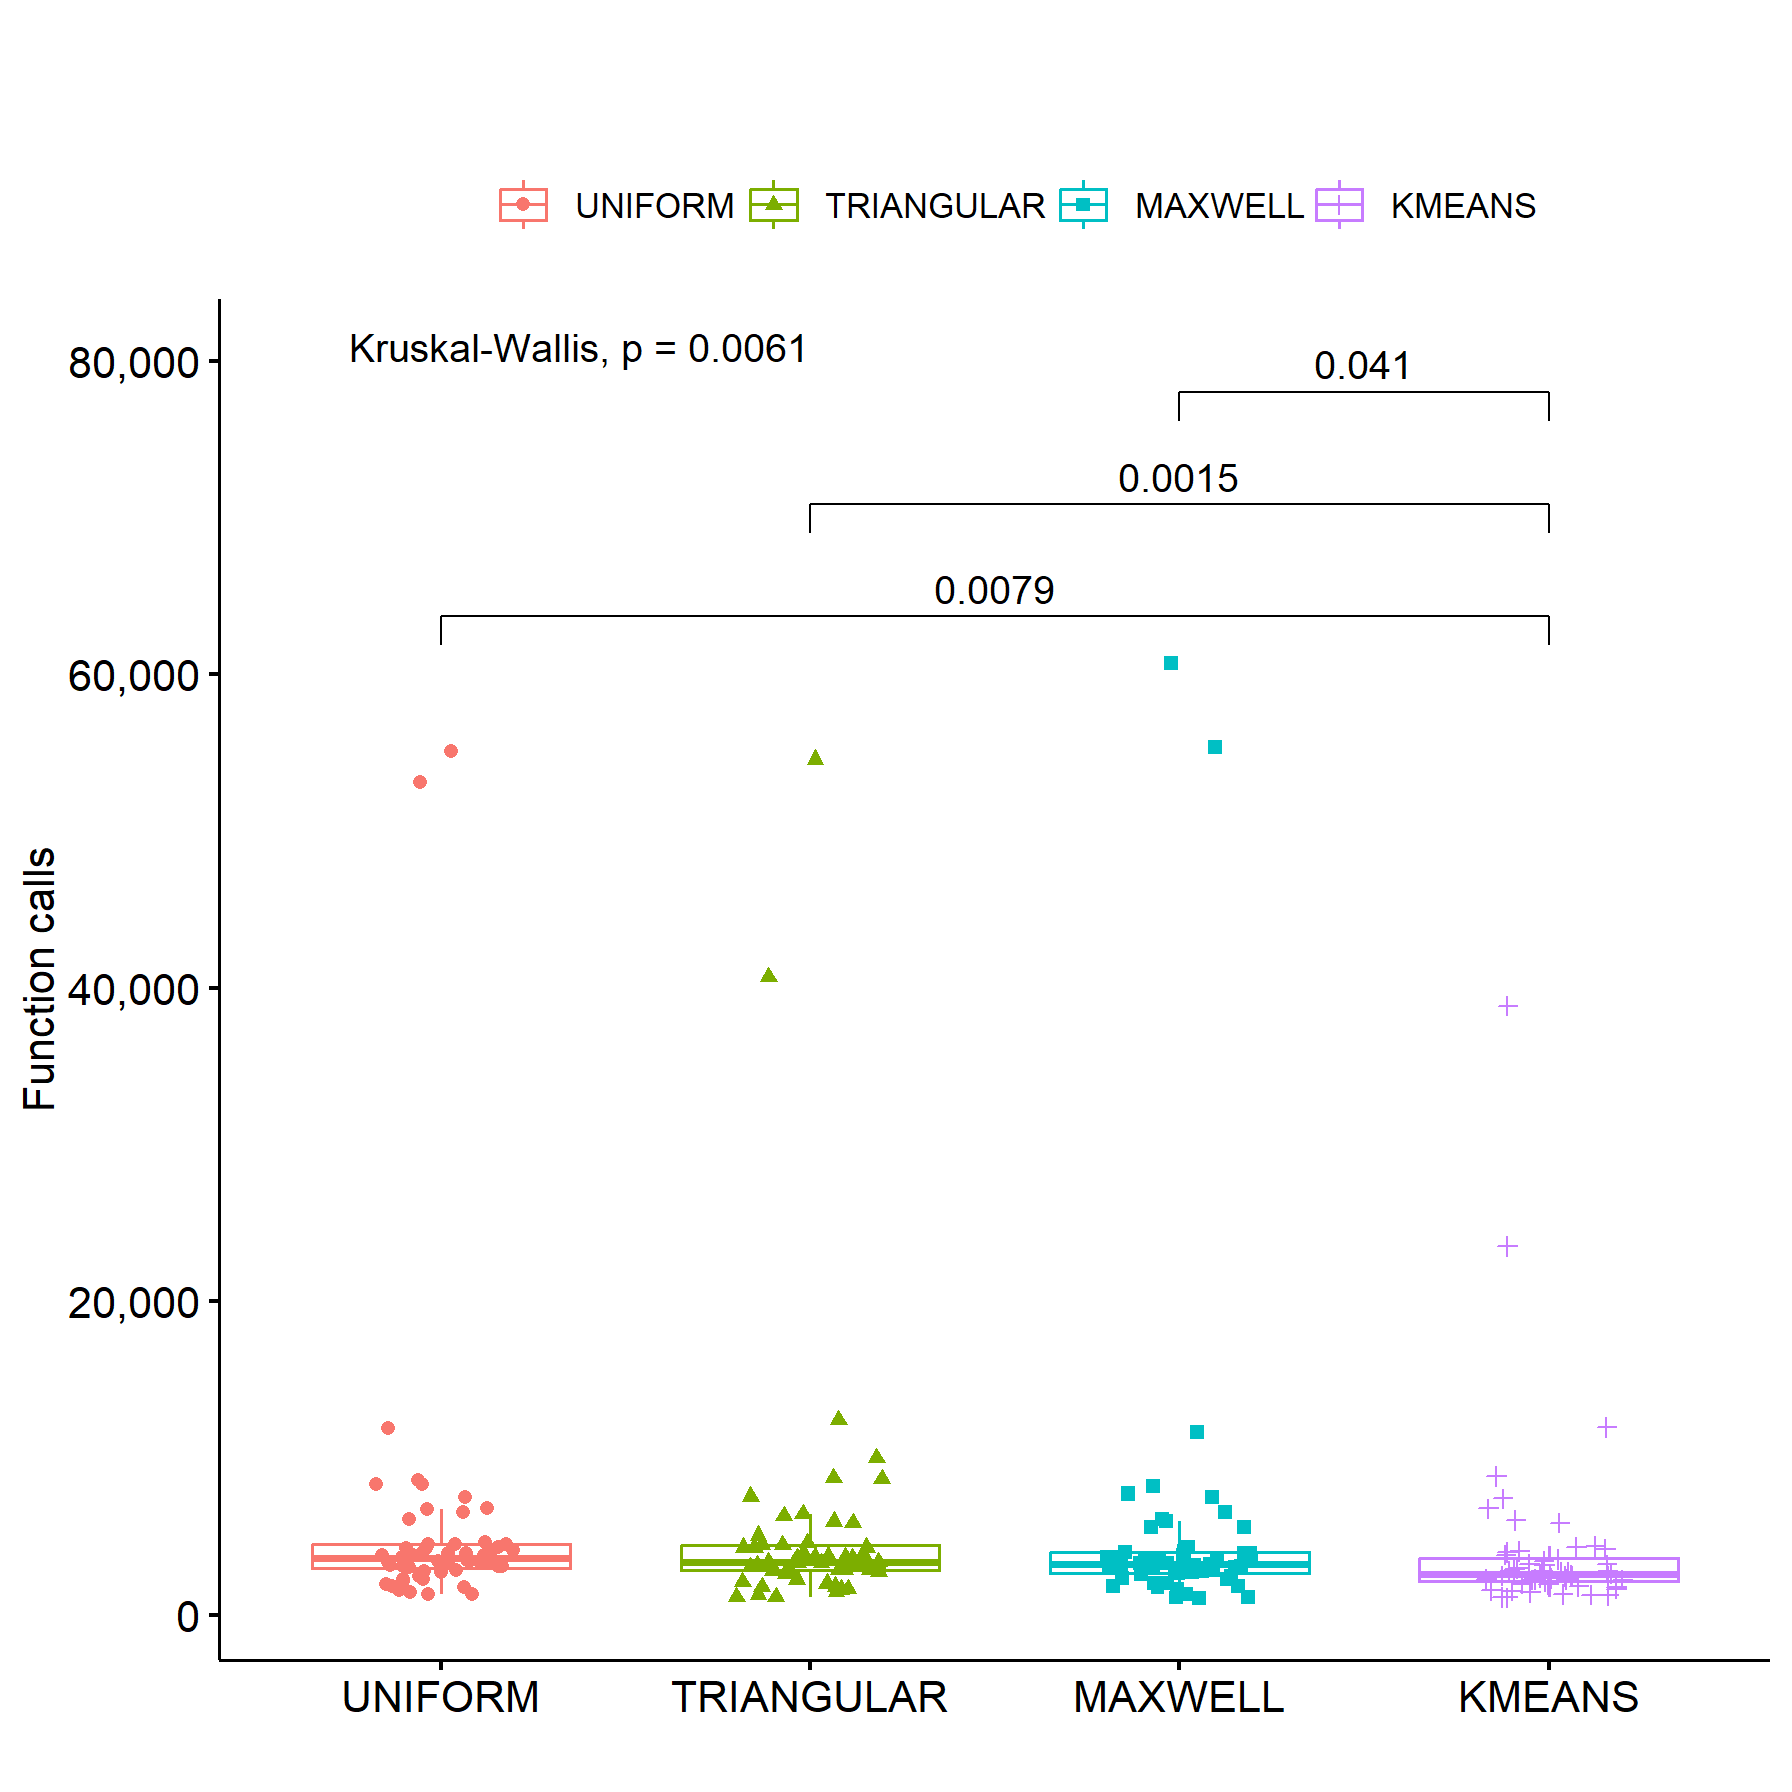
\includegraphics[scale=0.5]{image3}\caption{Scatter plot for different initial distributions\label{fig:ScatterPlot}}
\end{figure}
 

In addition, in order to investigate the impact that the choice of
sampling method has on the optimization method, an additional experiment
was done, in which the execution time of the proposed method was recorded
and with different sampling techniques for the ELP function, in which
function the dimension varied between 5 and 50. This function is defined
as:

\[
f(x)=\sum_{i=1}^{n}\left(10^{6}\right)^{\frac{i-1}{n-1}}x_{i}^{2}
\]
where the parameter $n$ defines the dimension of the function. The
results from this experiment are graphically outlined in Figure \ref{fig:timeComparison}.

\begin{figure}[H]
\begin{centering}
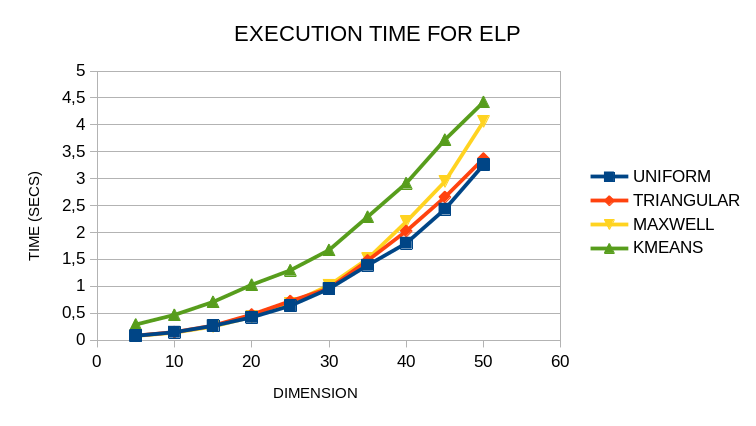
\includegraphics[scale=0.5]{elp_time_plot}
\par\end{centering}
\caption{Time comparison for the ELP function and the proposed optimization
method using the four sampling techniques mentioned before. The time
depicted in figure is the sum of the execution times for 30 independent
runs.\label{fig:timeComparison}}

\end{figure}
The proposed sampling method can significantly increase the required
execution time, since an iterative process is required before starting
the algorithm. The next sampling procedure in required execution time
appears to be the Maxwell sampling, but not significantly compared
to uniform sampling. 

\section{Conclusions \label{sec:Conclusions}}

The article proposed some modifications to the EEGO optimization method,
aimed to improve the overall performance and reduce the needed function
calls to discover the global minimum. The first modification concerns
the application of a sampling technique based on the K-Means method.
This technique allowed us to significantly minimize the number of
function calls to find the global minimum and further improved the
accuracy with which it is located. In particular, the application
of the K-Means method accelerated the finding of a solution, as it
more efficiently located the points of interest in the search space
and led to the fastest convergence to the global minimum. Compared
to other methods based on random distributions, the proposed technique
proved its superiority, especially in multidimensional and complex
functions.

The second proposed amendment concerns the termination rule based
on similarity of solutions during iterations. The main purpose of
this rule is to stop the optimization process when the iterated solutions
are too close to each other, thus preventing pointless iterations
that do not provide any significant improvement. It therefore avoids
wasting computing time in cases where the process is already very
close to the desired result. The use of the termination rule significantly
improves the efficiency of the algorithm.

Furthermore, one more improvement was suggested in this research paper.
This optimization adds randomness to the generation of new candidate
solutions from the old ones aiming to better explore the search space
of the objective problem in search of the global minimum. 

To verify the effectiveness of the new method, a series of experiments
were performed on a large group of objective problems from the recent
literature. In these experiments both the efficiency and speed improvement
of the original technique was measured and a comparison of the speed
of the new method was made in relation to other known techniques from
the relevant literature. Furthermore, a series of extensive experiments
were carried out to study the dynamics of the proposed initialization
technique as well as the additional time required by its implementation.
A number of useful conclusions were drawn from the execution of these
experiments. First of all, the new method significantly improves the
efficiency and speed of the original method. Furthermore, the experiments
revealed that the new method requires a significantly lower number
of function calls on average than other global optimization methods.
In addition, the sampling method proved to be highly efficient in
finding the global minimum and significantly reduced the required
number of function calls compared to other initialization techniques.
The additional time required by the new initialization method is noticeable
compared to other techniques but the gains it brings are equally significant. 

Future extensions of the proposed technique could be the use of parallel
programming techniques to speed up the overall process, such as the
MPI programming technique \citep{MPI} or the integration of the OpenMP
library \citep{OPENMP}, as well as the use of other termination techniques
that could potentially speed up the termination of the method. 

\vspace{6pt}


\authorcontributions{G.K., V.C. and I.G.T. created the software. G.K. conducted the experiments,
using a series of objective functions from various sources. V.C. conducted
the needed statistical tests. All authors have read and agreed to
the published version of the manuscript.}

\funding{This research received no external funding.}

\institutionalreview{Not applicable.}

\informedconsent{Not applicable.}

\dataavailability{The original contributions presented in the study are included in
the article, further inquiries can be directed to the corresponding
author.}

\acknowledgments{This research has been financed by the European Union: Next Generation
EU through the Program Greece 2.0 National Recovery and Resilience
Plan, under the call RESEARCH--CREATE--INNOVATE, project name “iCREW:
Intelligent small craft simulator for advanced crew training using
Virtual Reality techniques” (project code: TAEDK-06195).}

\conflictsofinterest{The authors declare no conflicts of interest.}

\appendixtitles{no}

\appendixstart{}

\appendix

\begin{adjustwidth}{-\extralength}{0cm}{}

\reftitle{References}
\begin{thebibliography}{999}
\bibitem{plhroforikh}Törn, A., Ali, M. M., \& Viitanen, S. (1999).
Stochastic global optimization: Problem classes and solution techniques.
Journal of Global Optimization, 14, 437-447.

\bibitem{computer}Floudas, C. A., \& Pardalos, P. M. (2013). State
of the art in global optimization: computational methods and applications

\bibitem{computer1}Horst, R., \& Pardalos, P. M. (2013). Handbook
of global optimization (Vol. 2). Springer Science \& Business Media.

\bibitem{maths}Intriligator, M. D. (2002). Mathematical optimization
and economic theory. Society for Industrial and Applied Mathematics.

\bibitem{maths-1}Cánovas, M. J., Kruger, A., Phu, H. X., \& Théra,
M. (2020). Marco A. López, a Pioneer of Continuous Optimization in
Spain. Vietnam Journal of Mathematics, 48, 211-219.

\bibitem{maths2}Mahmoodabadi, M. J., \& Nemati, A. R. (2016). A novel
adaptive genetic algorithm for global optimization of mathematical
test functions and real-world problems. Engineering Science and Technology,
an International Journal, 19(4), 2002-2021.

\bibitem{key-maths3}Li, J., Xiao, X., Boukouvala, F., Floudas, C.
A., Zhao, B., Du, G., ... \& Liu, H. (2016). Data‐driven mathematical
modeling and global optimization framework for entire petrochemical
planning operations. AIChE Journal, 62(9), 3020-3040.

\bibitem{fusikh}Iuliano, E. (2017). Global optimization of benchmark
aerodynamic cases using physics-based surrogate models. Aerospace
Science and Technology, 67, 273-286.

\bibitem{fusikh1}Duan, Q., Sorooshian, S., \& Gupta, V. (1992). Effective
and efficient global optimization for conceptual rainfall‐runoff models.
Water resources research, 28(4), 1015-1031.

\bibitem{fysikhh}Yang, L., Robin, D., Sannibale, F., Steier, C.,
\& Wan, W. (2009). Global optimization of an accelerator lattice using
multiobjective genetic algorithms. Nuclear Instruments and Methods
in Physics Research Section A: Accelerators, Spectrometers, Detectors
and Associated Equipment, 609(1), 50-57.

\bibitem{xhmeia}Heiles, S., \& Johnston, R. L. (2013). Global optimization
of clusters using electronic structure methods. International Journal
of Quantum Chemistry, 113(18), 2091-2109.

\bibitem{xhmeia1}Shin, W. H., Kim, J. K., Kim, D. S., \& Seok, C.
(2013). GalaxyDock2: Protein--ligand docking using beta‐complex and
global optimization. Journal of computational chemistry, 34(30), 2647-2656.

\bibitem{xhmeia2}Liwo, A., Lee, J., Ripoll, D. R., Pillardy, J.,
\& Scheraga, H. A. (1999). Protein structure prediction by global
optimization of a potential energy function. Proceedings of the National
Academy of Sciences, 96(10), 5482-5485.

\bibitem{iatrikh}Lee, E. K. (2007). Large-scale optimization-based
classification models in medicine and biology. Annals of biomedical
engineering, 35, 1095-1109.

\bibitem{iatrikh1}Cherruault, Y. (1994). Global optimization in biology
and medicine. Mathematical and computer modelling, 20(6), 119-132.

\bibitem{medicine}Houssein, E. H., Hosney, M. E., Mohamed, W. M.,
Ali, A. A., \& Younis, E. M. (2023). Fuzzy-based hunger games search
algorithm for global optimization and feature selection using medical
data. Neural Computing and Applications, 35(7), 5251-5275.

\bibitem{determistic}Ion, I. G., Bontinck, Z., Loukrezis, D., Römer,
U., Lass, O., Ulbrich, S., ... \& De Gersem, H. (2018). Robust shape
optimization of electric devices based on deterministic optimization
methods and finite-element analysis with affine parametrization and
design elements. Electrical Engineering, 100(4), 2635-2647.

\bibitem{determistic1}Cuevas-Velásquez, V., Sordo-Ward, A., García-Palacios,
J. H., Bianucci, P., \& Garrote, L. (2020). Probabilistic model for
real-time flood operation of a dam based on a deterministic optimization
model. Water, 12(11), 3206.

\bibitem{determistic2}Pereyra, M., Schniter, P., Chouzenoux, E.,
Pesquet, J. C., Tourneret, J. Y., Hero, A. O., \& McLaughlin, S. (2015).
A survey of stochastic simulation and optimization methods in signal
processing. IEEE Journal of Selected Topics in Signal Processing,
10(2), 224-241.

\bibitem{stohastic}Hannah, L. A. (2015). Stochastic optimization.
International Encyclopedia of the Social \& Behavioral Sciences, 2,
473-481.

\bibitem{stohastic1}Kizielewicz, B., \& Sałabun, W. (2020). A new
approach to identifying a multi-criteria decision model based on stochastic
optimization techniques. Symmetry, 12(9), 1551.

\bibitem{stohastic2}Chen, T., Sun, Y., \& Yin, W. (2021). Solving
stochastic compositional optimization is nearly as easy as solving
stochastic optimization. IEEE Transactions on Signal Processing, 69,
4937-4948.

\bibitem{key-1}Wolfe, M. A. (1996). Interval methods for global optimization.
Applied Mathematics and Computation, 75(2-3), 179-206.

\bibitem{interval2}Csendes, T., \& Ratz, D. (1997). Subdivision direction
selection in interval methods for global optimization. SIAM Journal
on Numerical Analysis, 34(3), 922-938.

\bibitem{Sergeyev}Sergeyev, Y. D., Kvasov, D. E., \& Mukhametzhanov,
M. S. (2018). On the efficiency of nature-inspired metaheuristics
in expensive global optimization with limited budget. Scientific reports,
8(1), 453.

\bibitem{diffe1}Storn, R., \& Price, K. (1997). Differential evolution--a
simple and efficient heuristic for global optimization over continuous
spaces. Journal of global optimization, 11, 341-359.

\bibitem{diffe2}Liu, J., \& Lampinen, J. (2005). A fuzzy adaptive
differential evolution algorithm. Soft Computing, 9, 448-462.

\bibitem{pso_major}Kennedy, J., \& Eberhart, R. (1995). Particle
swarm optimization. In Proceedings of ICNN'95-international conference
on neural networks (Vol. 4, pp. 1942-1948). ieee.

\bibitem{pso1}Poli, R., Kennedy, J., \& Blackwell, T. (2007). Particle
swarm optimization: An overview. Swarm intelligence, 1, 33-57.

\bibitem{pso2}Trelea, I. C. (2003). The particle swarm optimization
algorithm: convergence analysis and parameter selection. Information
processing letters, 85(6), 317-325.

\bibitem{aco1}Dorigo, M., Birattari, M., \& Stutzle, T. (2006). Ant
colony optimization. IEEE computational intelligence magazine, 1(4),
28-39.

\bibitem{aco2}Socha, K., \& Dorigo, M. (2008). Ant colony optimization
for continuous domains. European journal of operational research,
185(3), 1155-1173.

\bibitem{genetic1}Goldberg, D. E. (1989). Cenetic algorithms in search.
Optimization, Machine Learning.

\bibitem{genetic2}Michalewicz, Z. (1999). Genetic Algorithms+ Data
Structures= Evolution Programs. Springer-Verlag, 1999. Google Scholar
Google Scholar Digital Library Digital Library.

\bibitem{edo}Abdel-Basset, M., El-Shahat, D., Jameel, M., \& Abouhawwash,
M. (2023). Exponential distribution optimizer (EDO): a novel math-inspired
algorithm for global optimization and engineering problems. Artificial
Intelligence Review, 56(9), 9329-9400.

\bibitem{bdo}Ma, L., Cheng, S., \& Shi, Y. (2020). Enhancing learning
efficiency of brain storm optimization via orthogonal learning design.
IEEE Transactions on Systems, Man, and Cybernetics: Systems, 51(11),
6723-6742.

\bibitem{gpu1}Zhou, Y., \& Tan, Y. (2009). GPU-based parallel particle
swarm optimization. In 2009 IEEE Congress on Evolutionary Computation
(pp. 1493-1500). IEEE.

\bibitem{gpu2}Dawson, L., \& Stewart, I. (2013). Improving Ant Colony
Optimization performance on the GPU using CUDA. In 2013 IEEE Congress
on Evolutionary Computation (pp. 1901-1908). IEEE.

\bibitem{gpu3}Barkalov, K., \& Gergel, V. (2016). Parallel global
optimization on GPU. Journal of Global Optimization, 66, 3-20.

\bibitem{swarm1}Hassanien, A. E., \& Emary, E. (2018). Swarm intelligence:
principles, advances, and applications. CRC press.

\bibitem{swarm2}Tang, J., Liu, G., \& Pan, Q. (2021). A review on
representative swarm intelligence algorithms for solving optimization
problems: Applications and trends. IEEE/CAA Journal of Automatica
Sinica, 8(10), 1627-1643.

\bibitem{swarm}Brezočnik, L., Fister Jr, I., \& Podgorelec, V. (2018).
Swarm intelligence algorithms for feature selection: a review. Applied
Sciences, 8(9), 1521.

\bibitem{APPS}Tang, J., Liu, G., \& Pan, Q. (2021). A review on representative
swarm intelligence algorithms for solving optimization problems: Applications
and trends. IEEE/CAA Journal of Automatica Sinica, 8(10), 1627-1643.

\bibitem{bacterial}Chu, Y., Mi, H., Liao, H., Ji, Z., \& Wu, Q. H.
(2008). A fast bacterial swarming algorithm for high-dimensional function
optimization. In 2008 IEEE congress on evolutionary computation (IEEE
world congress on computational intelligence) (pp. 3135-3140). IEEE.

\bibitem{fish}Neshat, M., Sepidnam, G., Sargolzaei, M., \& Toosi,
A. N. (2014). Artificial fish swarm algorithm: a survey of the state-of-the-art,
hybridization, combinatorial and indicative applications. Artificial
intelligence review, 42(4), 965-997.

\bibitem{dolphin}Wu, T. Q., Yao, M., \& Yang, J. H. (2016). Dolphin
swarm algorithm. Frontiers of Information Technology \& Electronic
Engineering, 17(8), 717-729.

\bibitem{WOA}Mirjalili, S., \& Lewis, A. (2016). The whale optimization
algorithm. Advances in engineering software, 95, 51-67.

\bibitem{WOA1}Nasiri, J., \& Khiyabani, F. M. (2018). A whale optimization
algorithm (WOA) approach for clustering. Cogent Mathematics \& Statistics,
5(1), 1483565.

\bibitem{WOA2}Gharehchopogh, F. S., \& Gholizadeh, H. (2019). A comprehensive
survey: Whale Optimization Algorithm and its applications. Swarm and
Evolutionary Computation, 48, 1-24.

\bibitem{WOA3}Wang, J., Bei, J., Song, H., Zhang, H., \& Zhang, P.
(2023). A whale optimization algorithm with combined mutation and
removing similarity for global optimization and multilevel thresholding
image segmentation. Applied Soft Computing, 137, 110130.

\bibitem{tunicate}Kaur, S., Awasthi, L. K., Sangal, A. L., \& Dhiman,
G. (2020). Tunicate Swarm Algorithm: A new bio-inspired based metaheuristic
paradigm for global optimization. Engineering Applications of Artificial
Intelligence, 90, 103541.

\bibitem{ssaa}Wan, Y., Mao, M., Zhou, L., Zhang, Q., Xi, X., \& Zheng,
C. (2019). A novel nature-inspired maximum power point tracking (MPPT)
controller based on SSA-GWO algorithm for partially shaded photovoltaic
systems. Electronics, 8(6), 680.

\bibitem{SSA}Mirjalili, S., Gandomi, A. H., Mirjalili, S. Z., Saremi,
S., Faris, H., \& Mirjalili, S. M. (2017). Salp Swarm Algorithm: A
bio-inspired optimizer for engineering design problems. Advances in
engineering software, 114, 163-191.

\bibitem{SSA1}Bairathi, D., \& Gopalani, D. (2019). Salp swarm algorithm
(SSA) for training feed-forward neural networks. In Soft Computing
for Problem Solving: SocProS 2017, Volume 1 (pp. 521-534). Springer
Singapore.

\bibitem{SSA2}Abualigah, L., Shehab, M., Alshinwan, M., \& Alabool,
H. (2020). Salp swarm algorithm: a comprehensive survey. Neural Computing
and Applications, 32(15), 11195-11215.

\bibitem{abc}Karaboga, D., \& Akay, B. (2009). A comparative study
of artificial bee colony algorithm. Applied mathematics and computation,
214(1), 108-132.

\bibitem{search algorithm} Abdullahi, M., Ngadi, M. A., Dishing,
S. I., Abdulhamid, S. I. M., \& Usman, M. J. (2020). A survey of symbiotic
organisms search algorithms and applications. Neural computing and
applications, 32(2), 547-566.

\bibitem{several metaheuristic algorithms }Ezugwu, A. E., Adeleke,
O. J., Akinyelu, A. A., \& Viriri, S. (2020). A conceptual comparison
of several metaheuristic algorithms on continuous optimisation problems.
Neural Computing and Applications, 32(10), 6207-6251.

\bibitem{mutualism-parasitism}Wang, Y., \& DeAngelis, D. L. (2012).
A mutualism-parasitism system modeling host and parasite withmutualism
at low density. Mathematical Biosciences \& Engineering, 9(2), 431-444.

\bibitem{mutualistic}Aubier, T. G., Joron, M., \& Sherratt, T. N.
(2017). Mimicry among unequally defended prey should be mutualistic
when predators sample optimally. The American Naturalist, 189(3),
267-282.

\bibitem{Competition in mutualistic systems}Addicott, J. F. (1985).
Competition in mutualistic systems. The biology of mutualism: ecology
and evolution. Croom Helm, London, UK, 217-247.

\bibitem{hunting between groupers and giant moray eels in the Red Sea}Bshary,
R., Hohner, A., Ait-el-Djoudi, K., \& Fricke, H. (2006). Interspecific
communicative and coordinated hunting between groupers and giant moray
eels in the Red Sea. PLoS biology, 4(12), e431.

\bibitem{Eel and grouper optimizer}Ali Mohammadzadeh, Seyedali Mirjalili.
(2024) Eel and grouper optimizer: a nature-inspired optimization algorithm.
Springer Science+Business Media, LLC, part of Springer Nature 2024

\bibitem{key-28}Gogu, A., Nace, D., Dilo, A., Meratnia, N., \& Ortiz,
J. H. (2012). Review of optimization problems in wireless sensor networks. Telecommunications
Networks---Current Status and Future Trends, 153-180.

\bibitem{key-29}Goudos, S. K., Boursianis, A. D., Mohamed, A. W.,
Wan, S., Sarigiannidis, P., Karagiannidis, G. K., \& Suganthan, P.
N. (2021). Large Scale Global Optimization Algorithms for IoT Networks:
A Comparative Study. In 2021 17th International Conference on Distributed
Computing in Sensor Systems (DCOSS) (pp. 272-279). IEEE.

\bibitem{key-30}Arayapan, K., \& Warunyuwong, P. (2009). Logistics
optimization: Application of optimization modeling in inbound logistics.

\bibitem{key-34}Singh, S. P., Dhiman, G., Juneja, S., Viriyasitavat,
W., Singal, G., Kumar, N., \& Johri, P. (2023). A New QoS Optimization
in IoT-Smart Agriculture Using Rapid Adaption Based Nature-Inspired
Approach. IEEE Internet of Things Journal.

\bibitem{key-35}Wang, H., \& Ersoy, O. K. (2005). A novel evolutionary
global optimization algorithm and its application in bioinformatics. ECE
Technical Reports, 65.

\bibitem{key-36}Cassioli, A., Di Lorenzo, D., Locatelli, M., Schoen,
F., \& Sciandrone, M. (2012). Machine learning for global optimization. Computational
Optimization and Applications, 51, 279-303.

\bibitem{key-37}Houssein, E. H., Helmy, B. E. D., Elngar, A. A.,
Abdelminaam, D. S., \& Shaban, H. (2021). An improved tunicate swarm
algorithm for global optimization and image segmentation. IEEE Access, 9,
56066-56092.

\bibitem{key-38}Torun, H. M., \& Swaminathan, M. (2019). High-dimensional
global optimization method for high-frequency electronic design. IEEE
Transactions on Microwave Theory and Techniques, 67(6), 2128-2142.

\bibitem{key-39}Wang, L., Kan, J., Guo, J., \& Wang, C. (2019). 3D
path planning for the ground robot with improved ant colony optimization. Sensors, 19(4),
815.

\bibitem{kmeans2}Arora, P., \& Varshney, S. (2016). Analysis of k-means
and k-medoids algorithm for big data. Procedia Computer Science, 78,
507-512.

\bibitem{kmeans-ereunhtikh-koinothta}Ahmed, M., Seraj, R., \& Islam,
S. M. S. (2020). The k-means algorithm: A comprehensive survey and
performance evaluation. Electronics, 9(8), 1295.

\bibitem{charilogis}Charilogis, V., \& Tsoulos, I. G. (2022). Toward
an ideal particle swarm optimizer for multidimensional functions.
Information, 13(5), 217.

\bibitem{MacQueen}Macqueen, J. (1967). Some methods for classification
and analysis of multivariate observations. In Proceedings of 5-th
Berkeley Symposium on Mathematical Statistics and Probability/University
of California Press.

\bibitem{gainit1}Maaranen, H., Miettinen, K., \& Mäkelä, M. M. (2004).
Quasi-random initial population for genetic algorithms. Computers
\& Mathematics with Applications, 47(12), 1885-1895.

\bibitem{gainit2}Paul, P. V., Dhavachelvan, P., \& Baskaran, R. (2013).
A novel population initialization technique for genetic algorithm.
In 2013 International Conference on Circuits, Power and Computing
Technologies (ICCPCT) (pp. 1235-1238). IEEE.

\bibitem{aliInit}Ali, M., Pant, M., \& Abraham, A. (2013). Unconventional
initialization methods for differential evolution. Applied Mathematics
and Computation, 219(9), 4474-4494.

\bibitem{bajerInit}Bajer, D., Martinović, G., \& Brest, J. (2016).
A population initialization method for evolutionary algorithms based
on clustering and Cauchy deviates. Expert Systems with Applications,
60, 294-310.

\bibitem{KazimipourInit}Kazimipour, B., Li, X., \& Qin, A. K. (2014).
A review of population initialization techniques for evolutionary
algorithms. In 2014 IEEE congress on evolutionary computation (CEC)
(pp. 2585-2592). IEEE.

\bibitem{kmeans1-1}Li, Y., \& Wu, H. (2012). A clustering method
based on K-means algorithm. Physics Procedia, 25, 1104-1109.

\bibitem{jainTermination}Jain, B. J., Pohlheim, H., \& Wegener, J.
(2001). On termination criteria of evolutionary algorithms. In Proceedings
of the 3rd Annual Conference on Genetic and Evolutionary Computation
(pp. 768-768).

\bibitem{zilTermination}Zielinski, K., Weitkemper, P., Laur, R.,
\& Kammeyer, K. D. (2006). Examination of stopping criteria for differential
evolution based on a power allocation problem. In Proceedings of the
10th International Conference on Optimization of Electrical and Electronic
Equipment (Vol. 3, pp. 149-156).

\bibitem{ghoreishiTermination}Ghoreishi, S. N., Clausen, A., \& Jørgensen,
B. N. (2017). Termination Criteria in Evolutionary Algorithms: A Survey.
In IJCCI (pp. 373-384).

\bibitem{ravberTermination}Ravber, M., Liu, S. H., Mernik, M., \&
Črepinšek, M. (2022). Maximum number of generations as a stopping
criterion considered harmful. Applied Soft Computing, 128, 109478.

\bibitem{key-1}Javad Ebadi, M., Fahs, A., Fahs, H., \& Dehghani,
R. (2023). Competitive secant (BFGS) methods based on modified secant
relations for unconstrained optimization. Optimization, 72(7), 1691-1706.

\bibitem{eofa}Kyrou, G., Charilogis, V., \& Tsoulos, I. G. (2024).
EOFA: An Extended Version of the Optimal Foraging Algorithm for Global
Optimization Problems. Computation, 12(8), 158.

\bibitem{newGA}Charilogis, V., Tsoulos, I. G., \& Stavrou, V. N.
(2023). An Intelligent Technique for Initial Distribution of Genetic
Algorithms. Axioms, 12(10), 980.

\bibitem{ppso}Charilogis, V., Tsoulos, I. G., \& Tzallas, A. (2023).
An improved parallel particle swarm optimization. SN Computer Science,
4(6), 766.

\bibitem{igao}Kyrou, G., Charilogis, V., \& Tsoulos, I. G. (2024).
Improving the Giant-Armadillo Optimization Method. Analytics, 3(2),
225-240.

\bibitem{kmeans-paterrn}Ali, H. H., \& Kadhum, L. E. (2017). K-means
clustering algorithm applications in data mining and pattern recognition.
International Journal of Science and Research (IJSR), 6(8), 1577-1584.

\bibitem{gen_kmeans}Krishna, K., \& Murty, M. N. (1999). Genetic
K-means algorithm. IEEE Transactions on Systems, Man, and Cybernetics,
Part B (Cybernetics), 29(3), 433-439.

\bibitem{unsuper_kmeans}Sinaga, K. P., \& Yang, M. S. (2020). Unsupervised
K-means clustering algorithm. IEEE access, 8, 80716-80727.

\bibitem{fixed_kmeans}Ay, M., Özbakır, L., Kulluk, S., Gülmez, B.,
Öztürk, G., \& Özer, S. (2023). FC-Kmeans: Fixed-centered K-means
algorithm. Expert Systems with Applications, 211, 118656.

\bibitem{kmeans_review}Oti, E. U., Olusola, M. O., Eze, F. C., \&
Enogwe, S. U. (2021). Comprehensive review of K-Means clustering algorithms.
criterion, 12, 22-23.

\bibitem{Ali}Ali, M. M., Khompatraporn, C., \& Zabinsky, Z. B. (2005).
A numerical evaluation of several stochastic algorithms on selected
continuous global optimization test problems. Journal of global optimization,
31, 635-672.

\bibitem{Floudas1}Floudas, C. A., Pardalos, P. M., Adjiman, C., Esposito,
W. R., Gümüs, Z. H., Harding, S. T., ... \& Schweiger, C. A. (2013).
Handbook of test problems in local and global optimization (Vol. 33).
Springer Science \& Business Media.

\bibitem{testfunc1}Ali, M. M., \& Kaelo, P. (2008). Improved particle
swarm algorithms for global optimization. Applied mathematics and
computation, 196(2), 578-593.

\bibitem{testfunc2}Koyuncu, H., \& Ceylan, R. (2019). A PSO based
approach: Scout particle swarm algorithm for continuous global optimization
problems. Journal of Computational Design and Engineering, 6(2), 129-142.

\bibitem{testfunc2-1}Siarry, P., Berthiau, G., Durdin, F., \& Haussy,
J. (1997). Enhanced simulated annealing for globally minimizing functions
of many-continuous variables. ACM Transactions on Mathematical Software
(TOMS), 23(2), 209-228.

\bibitem{testfunc3}Tsoulos, I. G., \& Lagaris, I. E. (2008). GenMin:
An enhanced genetic algorithm for global optimization. Computer Physics
Communications, 178(11), 843-851.

\bibitem{testfunc4}LaTorre, A., Molina, D., Osaba, E., Poyatos, J.,
Del Ser, J., \& Herrera, F. (2021). A prescription of methodological
guidelines for comparing bio-inspired optimization algorithms. Swarm
and Evolutionary Computation, 67, 100973.

\bibitem{gec}Li, X., Engelbrecht, A., \& Epitropakis, M. G. (2013).
Benchmark functions for CEC’2013 special session and competition on
niching methods for multimodal function optimization. RMIT University,
Evolutionary Computation and Machine Learning Group, Australia, Tech.
Rep.

\bibitem{gkls}Gaviano, M., Kvasov, D. E., Lera, D., \& Sergeyev,
Y. D. (2003). Algorithm 829: Software for generation of classes of
test functions with known local and global minima for global optimization.
ACM Transactions on Mathematical Software (TOMS), 29(4), 469-480

\bibitem{jones}Jones, J. E. (1924). On the determination of molecular
fields.---II. From the equation of state of a gas. Proceedings of
the Royal Society of London. Series A, Containing Papers of a Mathematical
and Physical Character, 106(738), 463-477.

\bibitem{powell}Powell, M.J.D. (1989). A Tolerant Algorithm for Linearly
Constrained Optimization Calculations. Math. Program, 45, 547--566.

\bibitem{doublepop}Tsoulos, I. G. (2008). Modifications of real code
genetic algorithm for global optimization. Applied Mathematics and
Computation, 203(2), 598-607.

\bibitem{ipso}Charilogis, V., \& Tsoulos, I. G. (2022). Toward an
ideal particle swarm optimizer for multidimensional functions. Information,
13(5), 217.

\bibitem{triangular}Stein, W. E., \& Keblis, M. F. (2009). A new
method to simulate the triangular distribution. Mathematical and Computer
Modelling, 49(5-6), 1143-1147.

\bibitem{maxwell}Sharma, V. K., Bakouch, H. S., \& Suthar, K. (2017).
An extended Maxwell distribution: Properties and applications. Communications
in Statistics-Simulation and Computation, 46(9), 6982-7007.

\bibitem[(2022)]{Browne}Browne, D. et al., (2022). Applications of
Uniform Distributions in Optimization Algorithms. Journal of Applied
Statistics, 45(2), 123-139.

\bibitem[(2023)]{Zhao}Zhao, Y., et al., (2023). Risk Management Models
Using Triangular Distributions. Risk Analysis Quarterly, 39(1), 98-112.

\bibitem[(2021)]{Chen}Chen, L., et al., (2021). Simulating Communication
Networks with Maxwell Distribution. IEEE Transactions on Communications,
68(4), 568-578.

\bibitem[(2022)]{Xu}Xu, J., et al., (2022). Improving K-means Clustering
with K-means++ Initialization. Machine Learning Journal, 34(3), 245-267.

\bibitem{MPI}Gropp, W., Lusk, E., Doss, N., \& Skjellum, A. (1996).
A high-performance, portable implementation of the MPI message passing
interface standard. Parallel computing, 22(6), 789-828.

\bibitem{OPENMP}Chandra, R. (2001). Parallel Programming in OpenMP.
Academic Press.

\bibitem{scaa}Gad, A. G. (2022). Particle swarm optimization algorithm
and its applications: a systematic review. Archives of computational
methods in engineering, 29(5), 2531-2561.

\end{thebibliography}
%%%%%%%%%%%%%%%%%%%%%%%%%%%%%%%%%%%%%%%%%%
%% for journal Sci
%\reviewreports{\\
%Reviewer 1 comments and authors' response\\
%Reviewer 2 comments and authors' response\\
%Reviewer 3 comments and authors' response
%}
%%%%%%%%%%%%%%%%%%%%%%%%%%%%%%%%%%%%%%%%%%

\PublishersNote{}

\end{adjustwidth}{}
\end{document}
